\chapter{Zeichnungen}\label{sec:zeichnungen}
\newpage
\setlength{\voffset}{0cm}
\setlength{\hoffset}{0cm}
\newpage
\setlength{\voffset}{-2.5 cm}
\setlength{\hoffset}{-2 cm}
\section{Bauteilzeichnungen}\label{sec:bauteilzeichnungen}
\newpage
\setlength{\voffset}{0cm}
\setlength{\hoffset}{0cm}
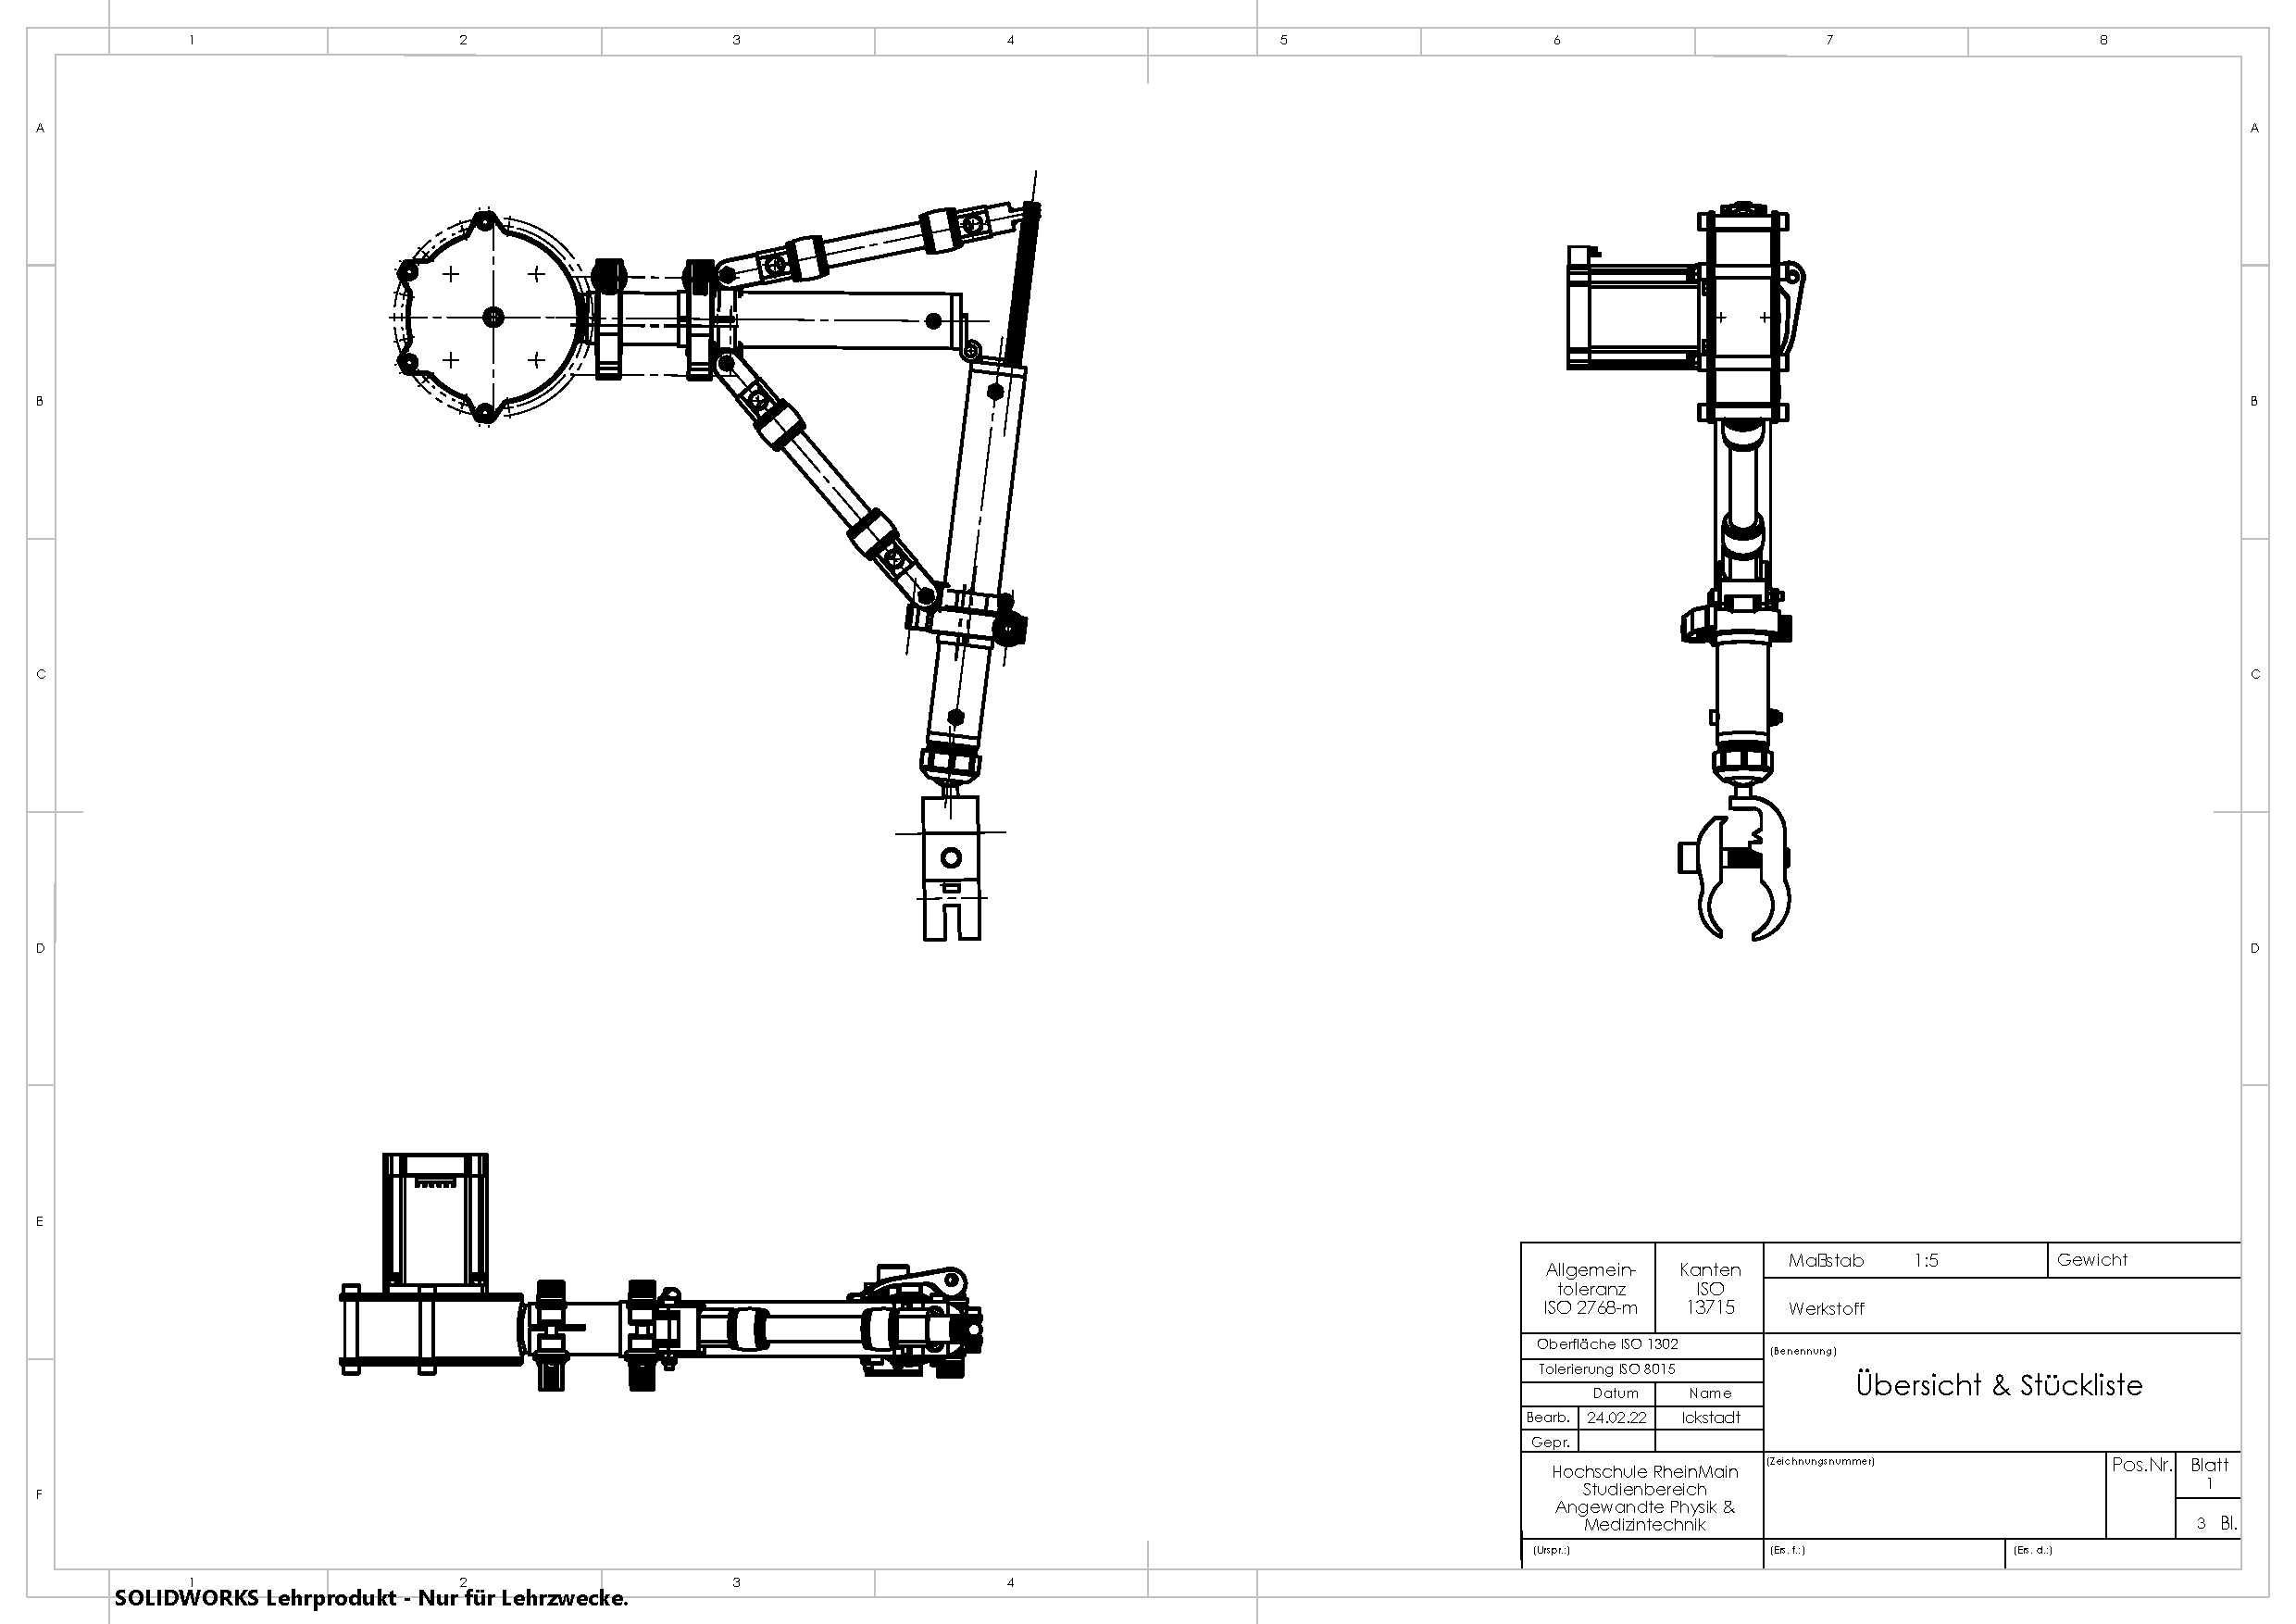
\includepdf[pages=1, angle=90, pagecommand={\thispagestyle{plain}}]{Abb/CAD/Drawings/Uebersicht-und-Stueckliste.pdf}
\includepdf[pages=2, angle=90, pagecommand={\thispagestyle{plain}}]{Abb/CAD/Drawings/Uebersicht-und-Stueckliste.pdf}
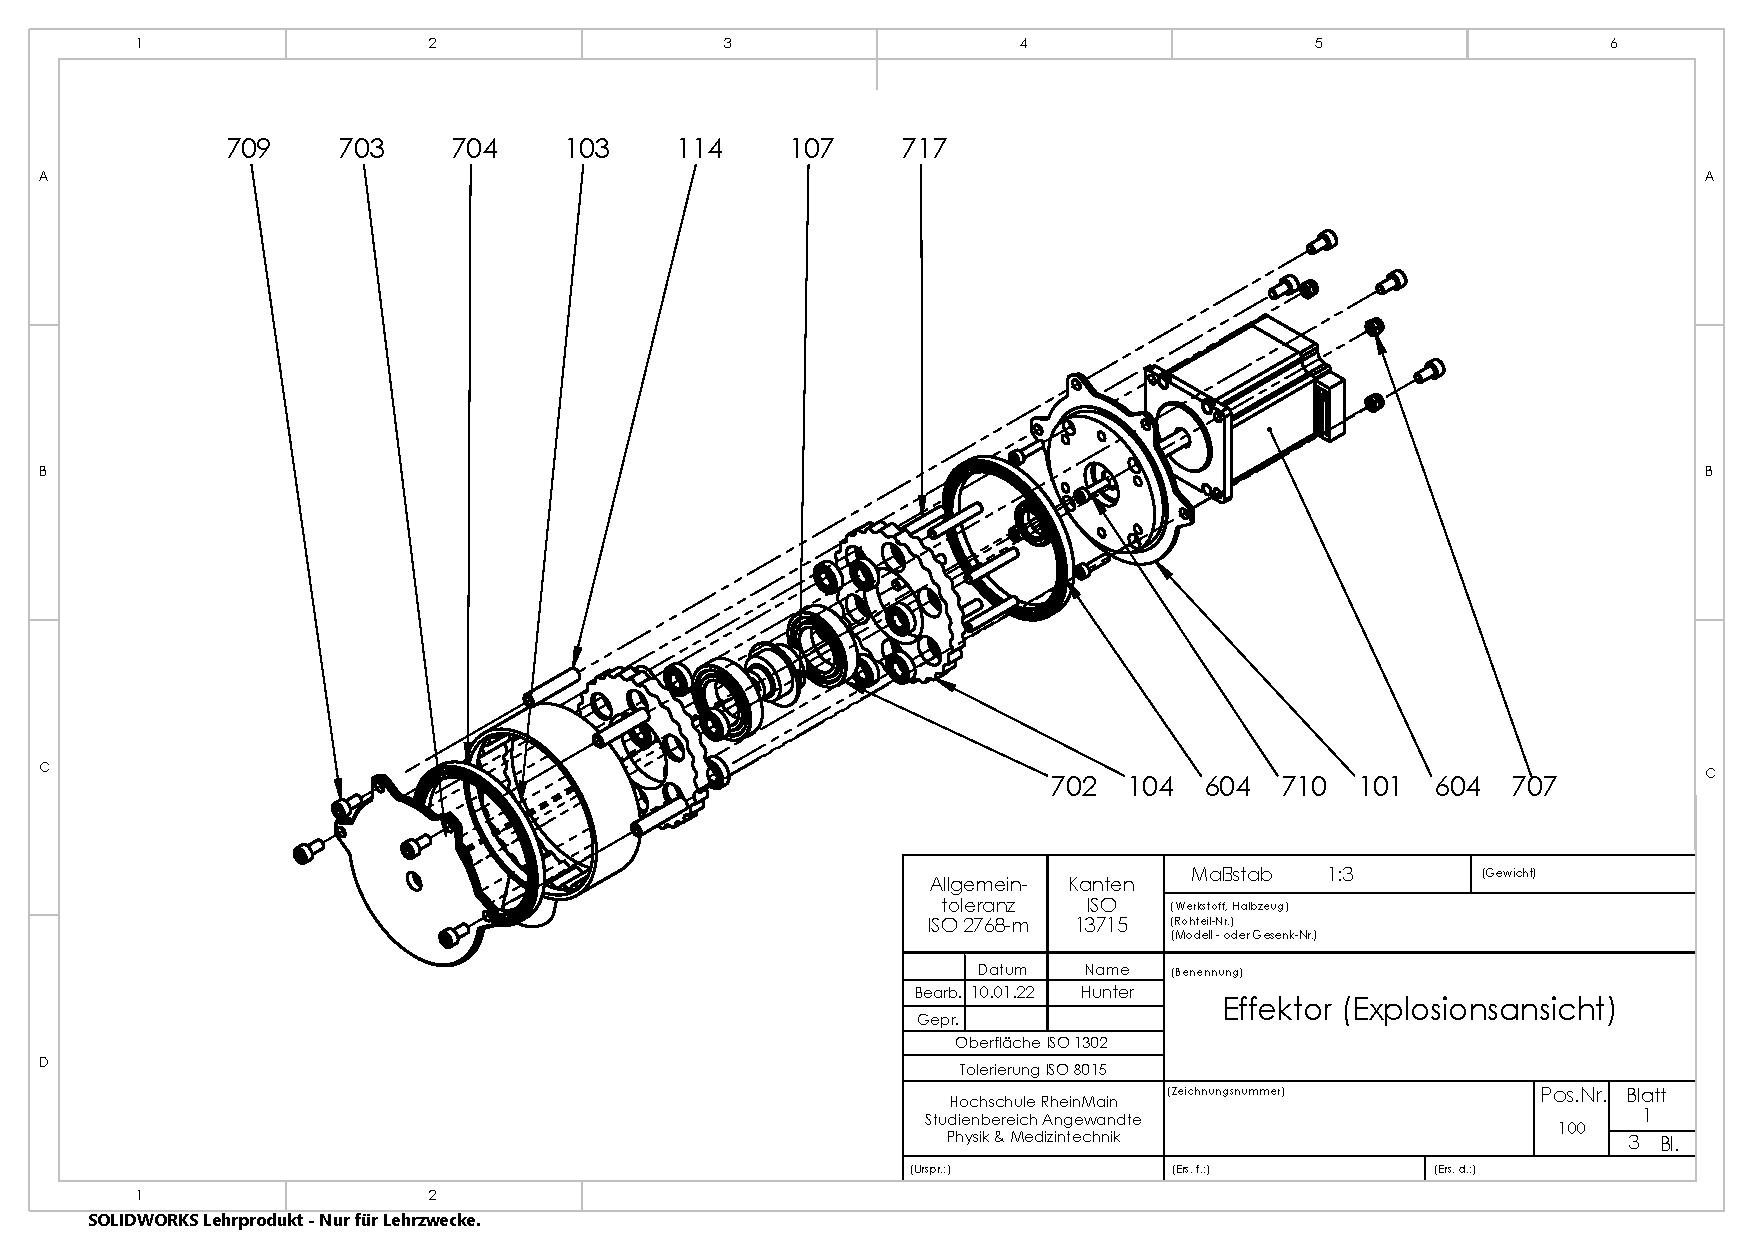
\includepdf[pages=1, angle=90, pagecommand={\thispagestyle{plain}}]{Abb/CAD/Drawings/Schulter/Effektor-assembly-drawing.pdf}
\includepdf[pages=2-3, angle=0, pagecommand={\thispagestyle{plain}}]{Abb/CAD/Drawings/Schulter/Effektor-assembly-drawing.pdf}
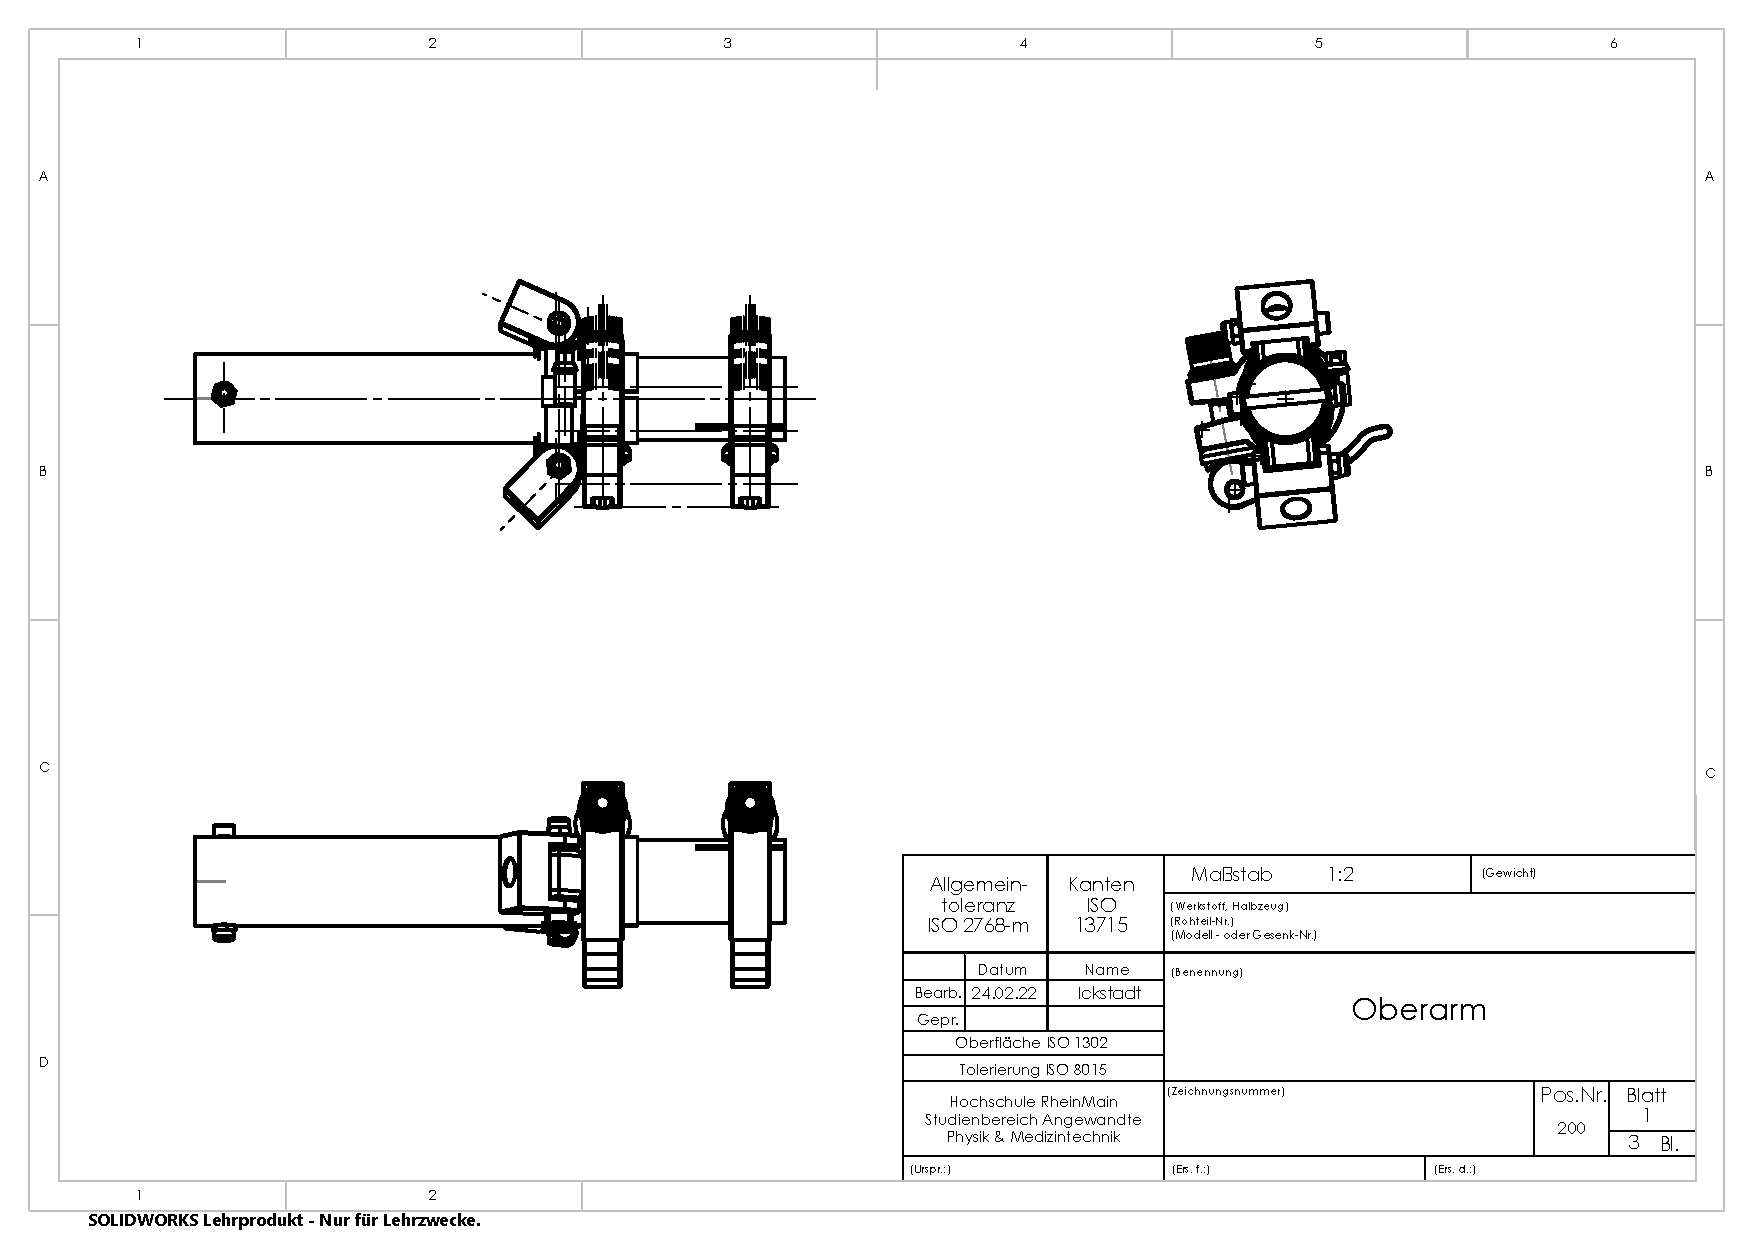
\includepdf[pages=1-2, angle=90, pagecommand={\thispagestyle{plain}}]{Abb/CAD/Drawings/Oberarm.pdf}
\includepdf[pages=3, angle=0, pagecommand={\thispagestyle{plain}}]{Abb/CAD/Drawings/Oberarm.pdf}
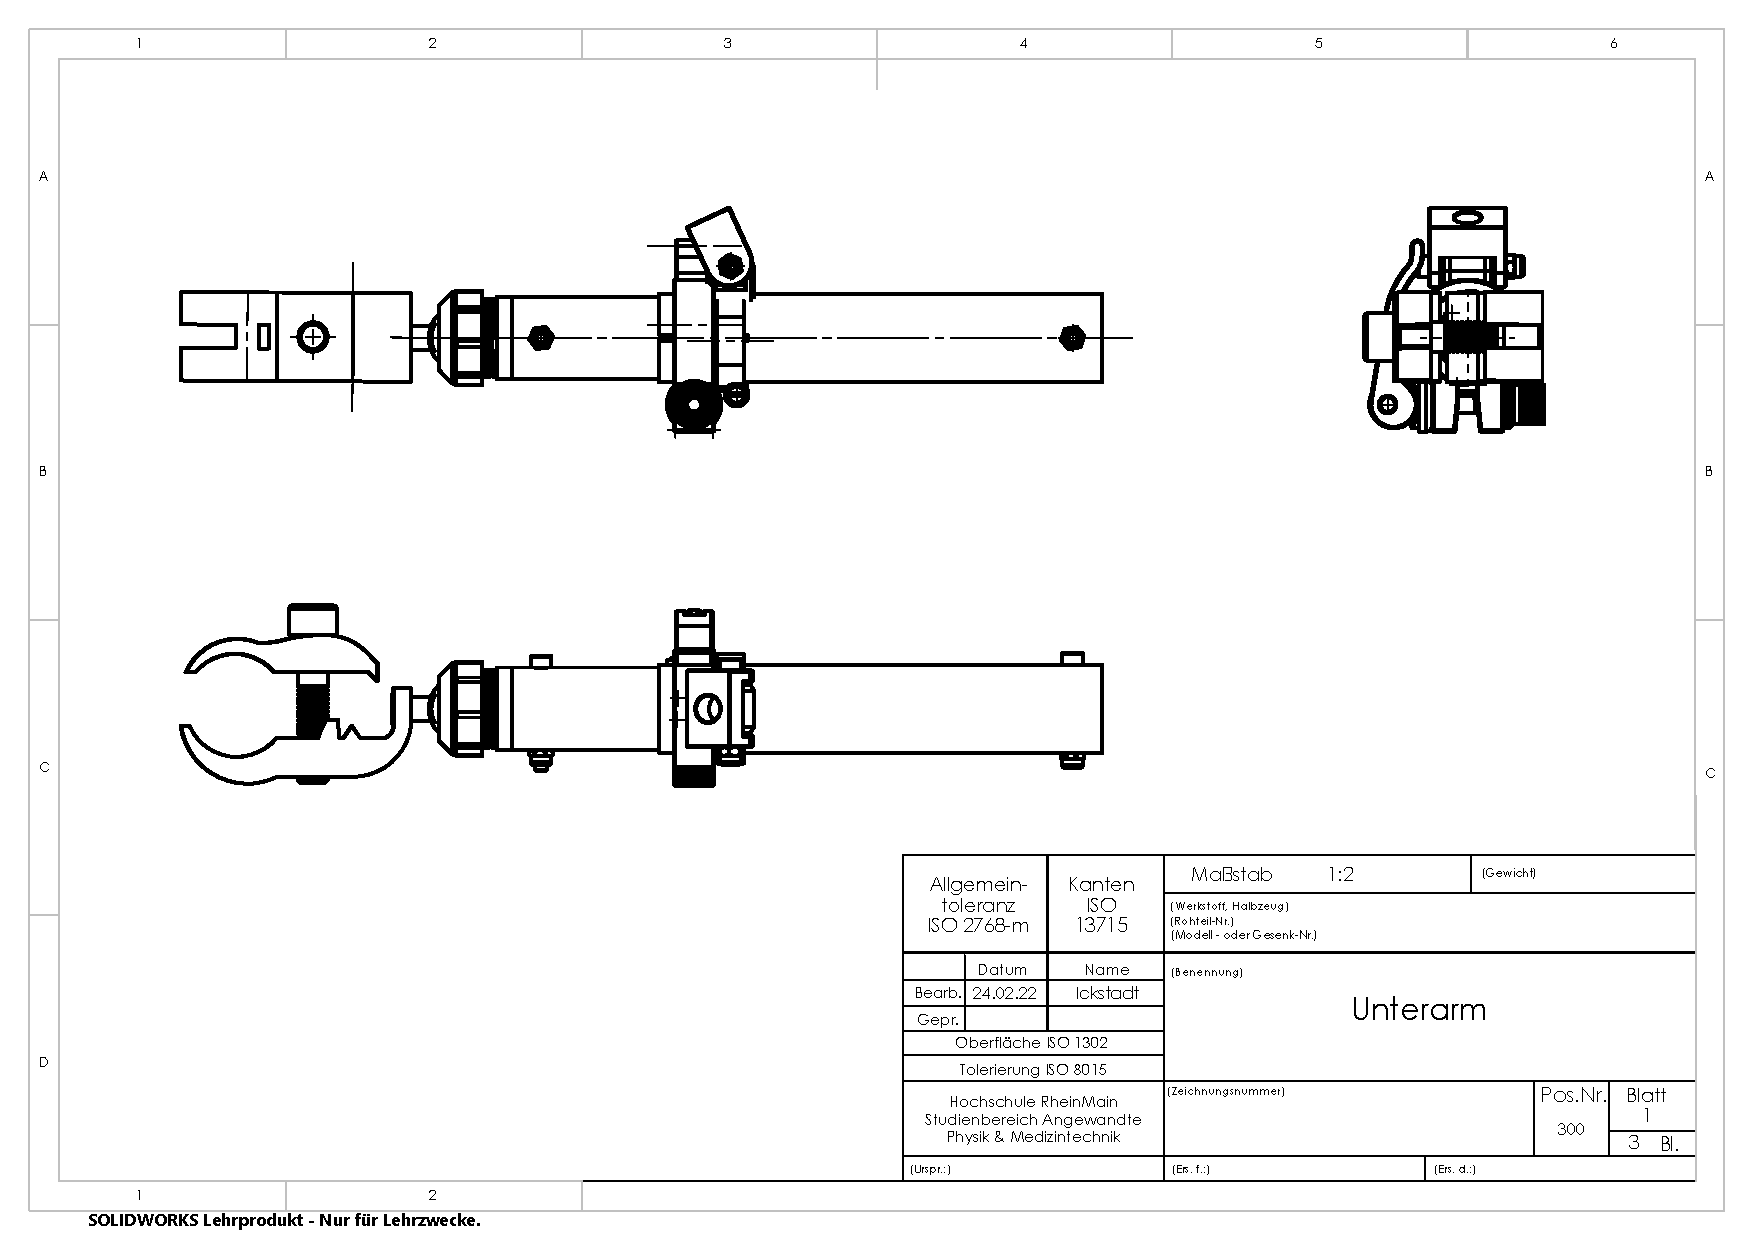
\includepdf[pages=1-2, angle=90, pagecommand={\thispagestyle{plain}}]{Abb/CAD/Drawings/Unterarm.pdf}
\includepdf[pages=3, angle=0, pagecommand={\thispagestyle{plain}}]{Abb/CAD/Drawings/Unterarm.pdf}
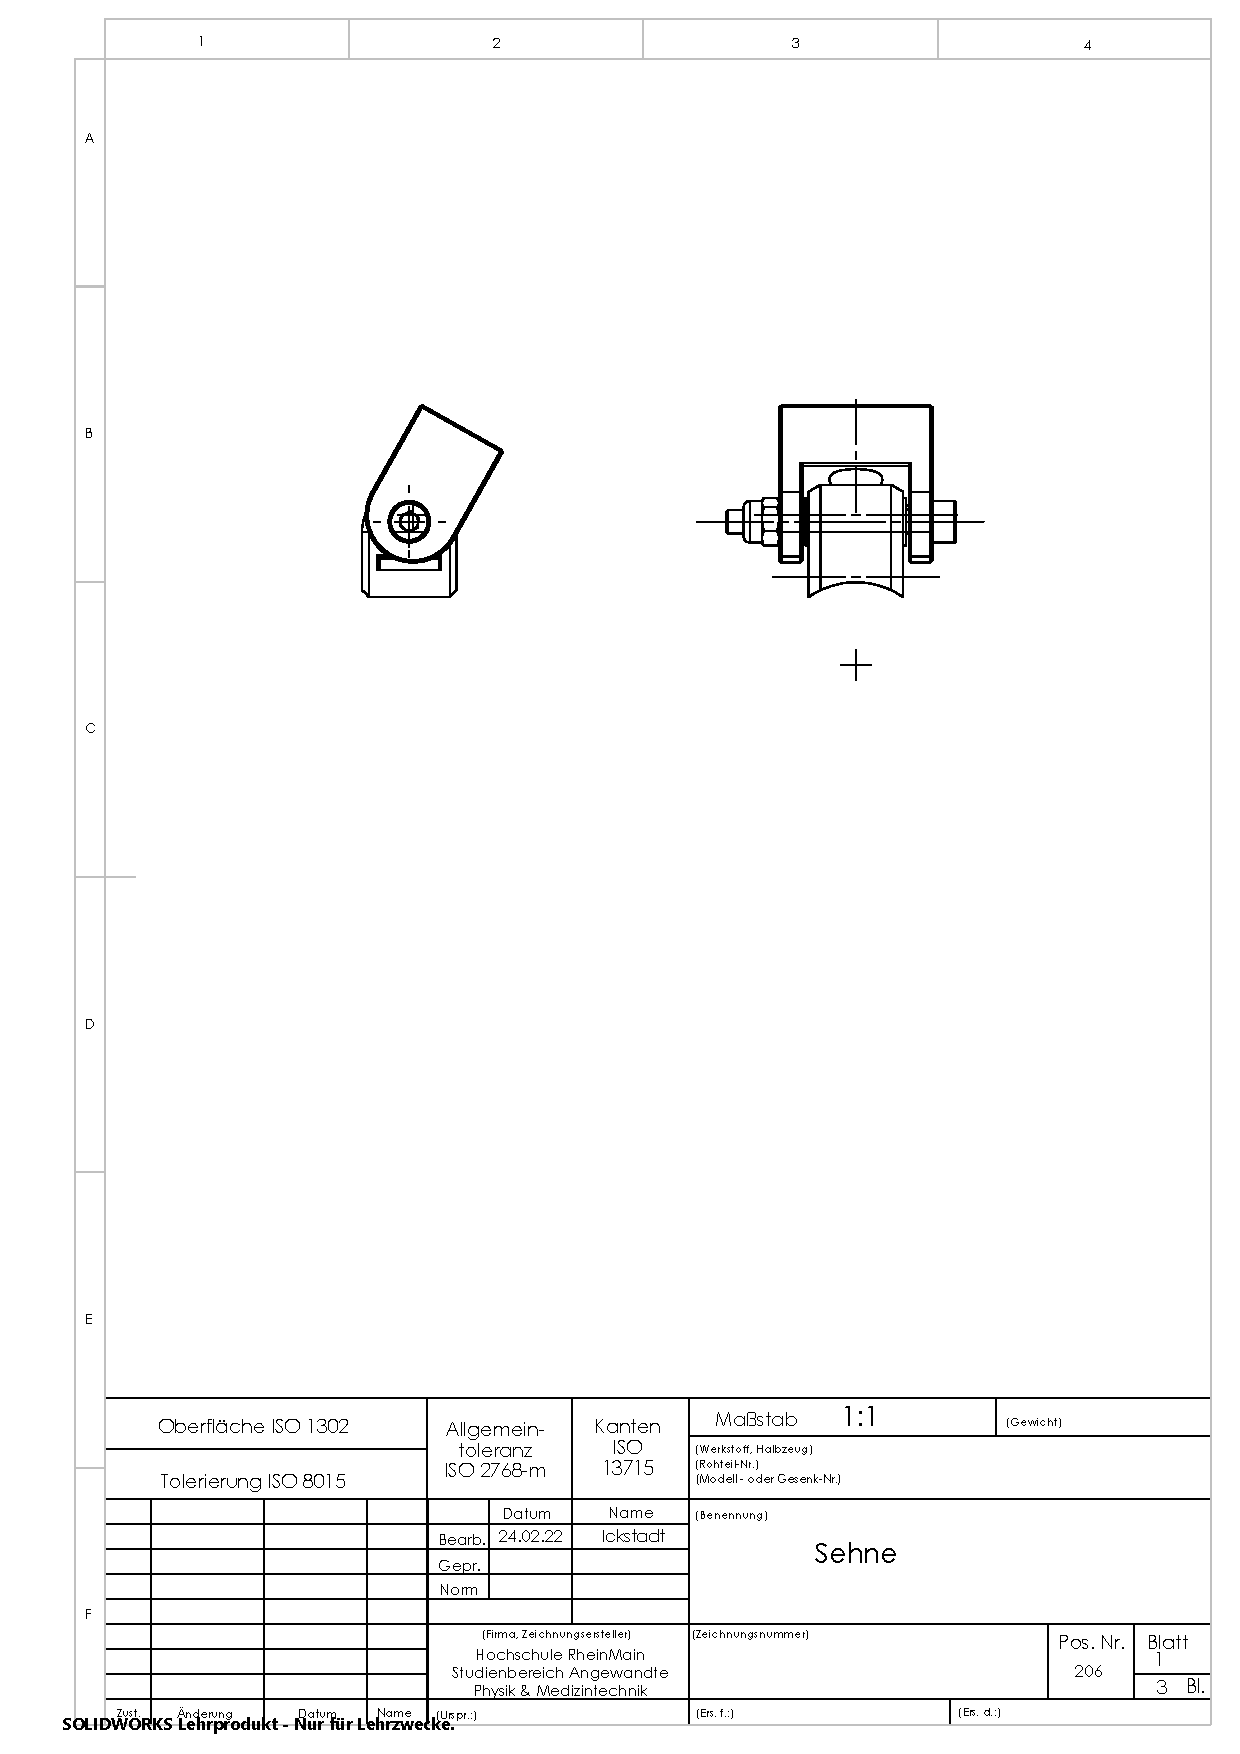
\includepdf[pages=-, angle=0, pagecommand={\thispagestyle{plain}}]{Abb/CAD/Drawings/Sehne.pdf}
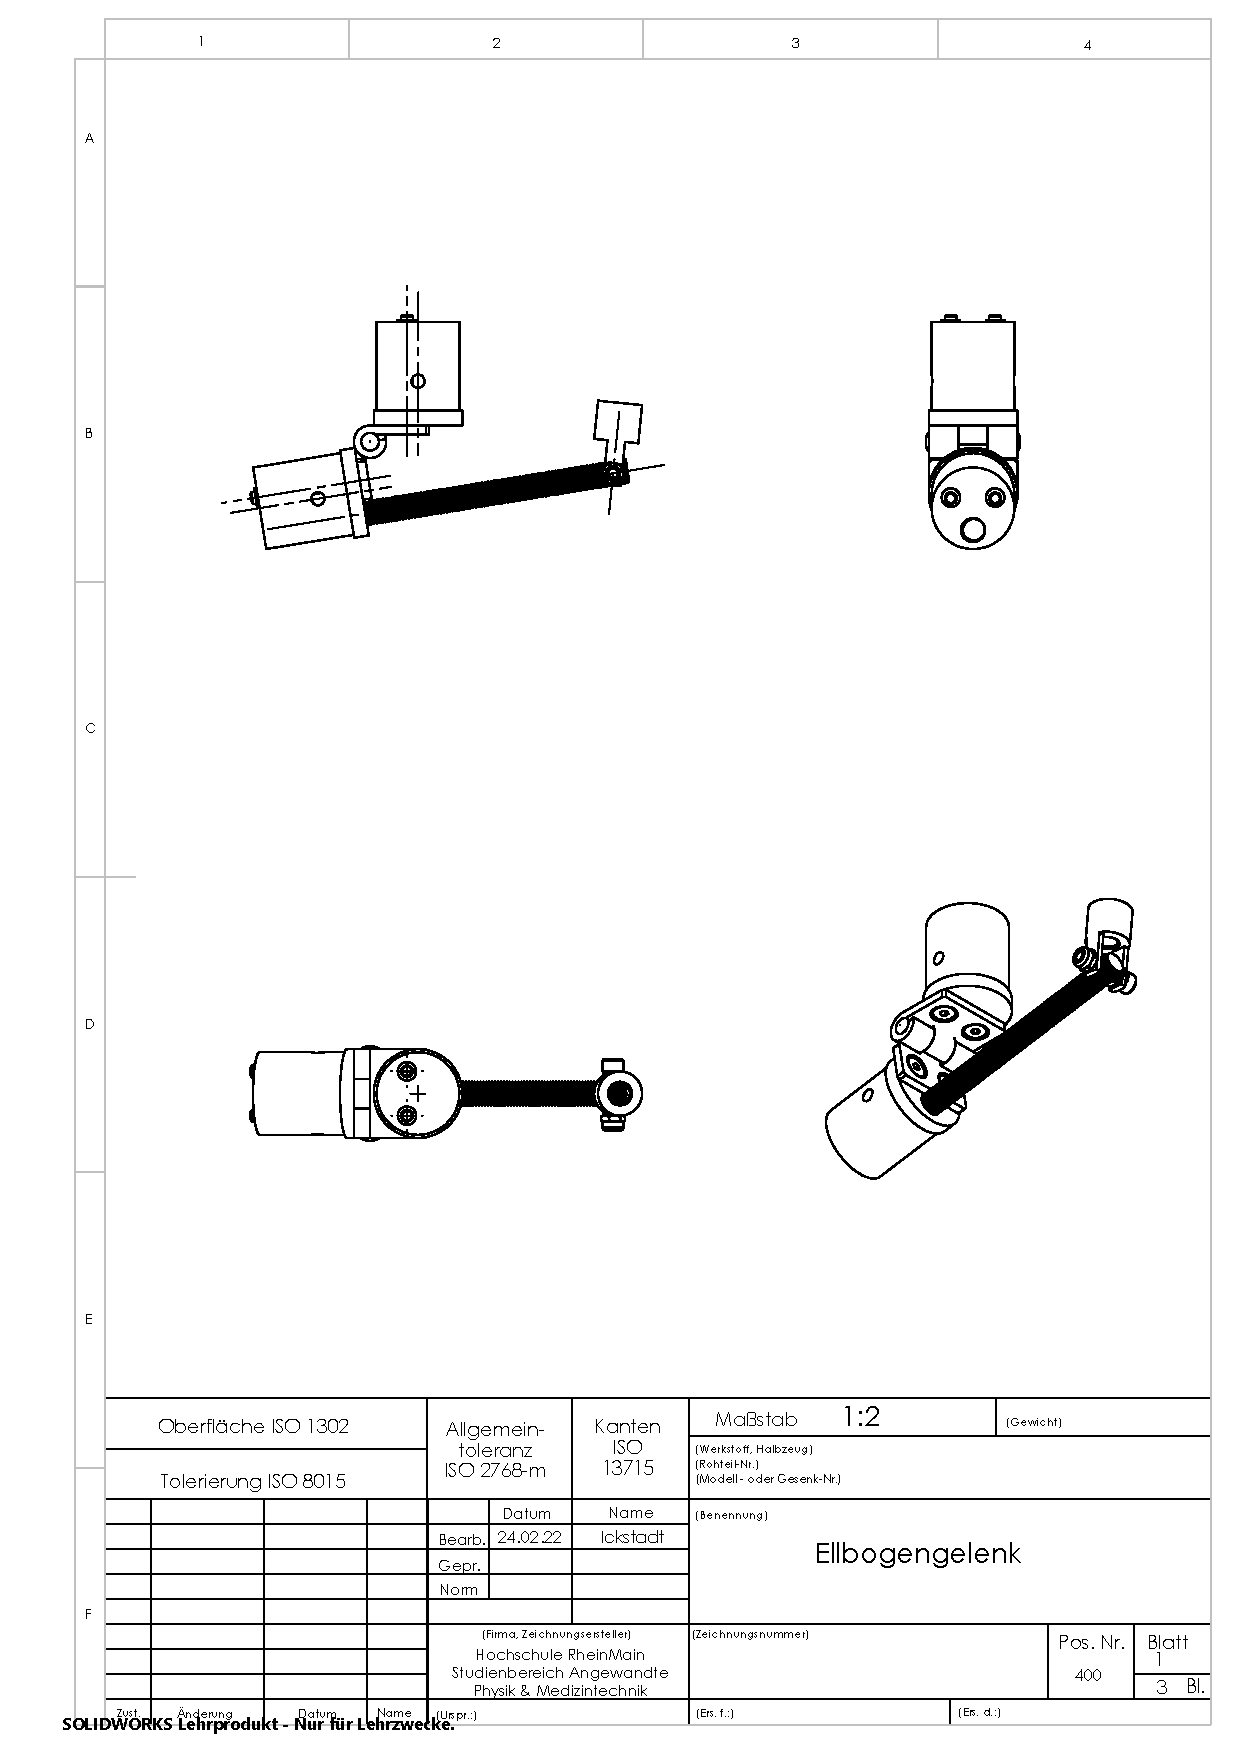
\includepdf[pages=-, angle=0, pagecommand={\thispagestyle{plain}}]{Abb/CAD/Drawings/Ellbogengelenk.pdf}
%
\newpage
\setlength{\voffset}{-2.5 cm}
\setlength{\hoffset}{-2 cm}
\section{Einzelteilzeichnungen Schultergelenk}\label{sec:einzelteilzeichnungen schultergelenk}
\newpage
\setlength{\voffset}{0cm}
\setlength{\hoffset}{0cm}
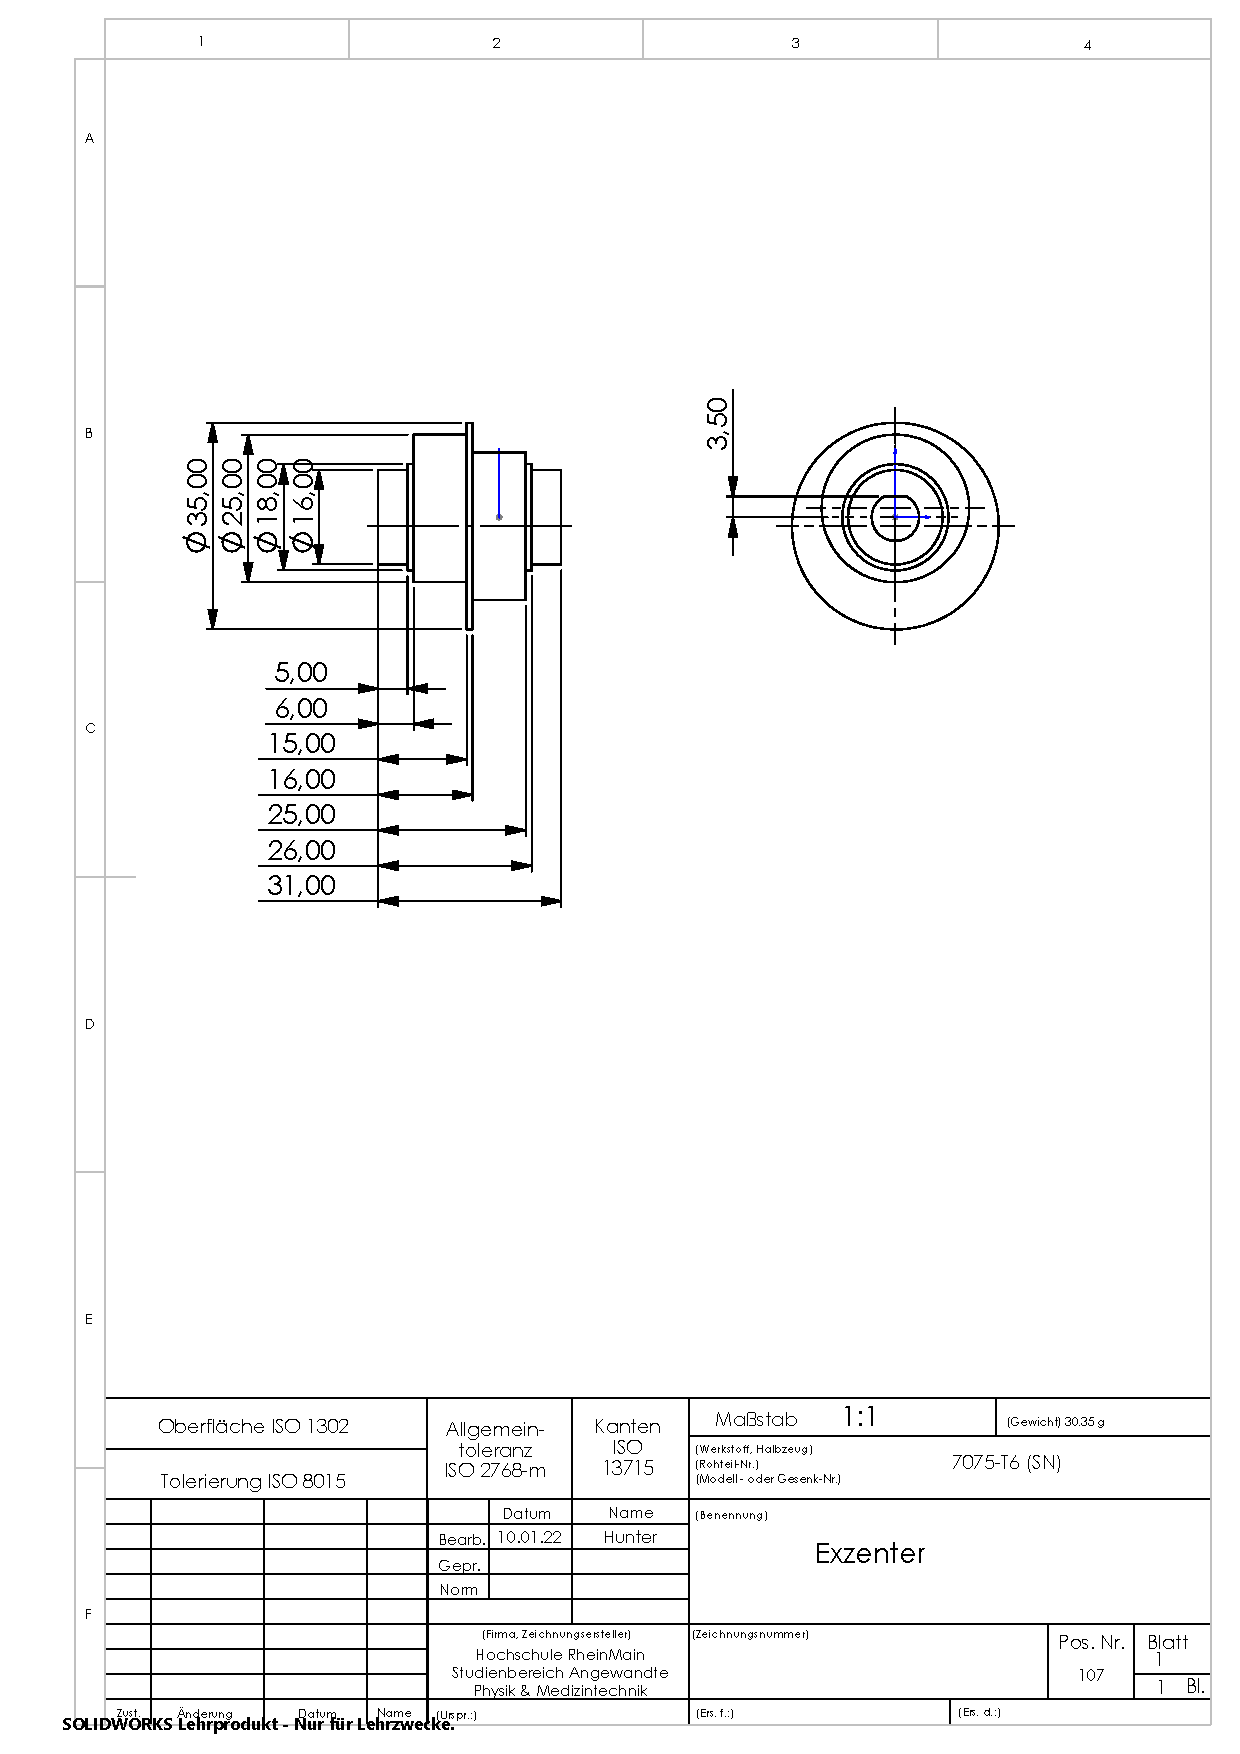
\includepdf[pages=-, angle=0, pagecommand={\thispagestyle{plain}}]{Abb/CAD/Drawings/Schulter/Exzenter.pdf}
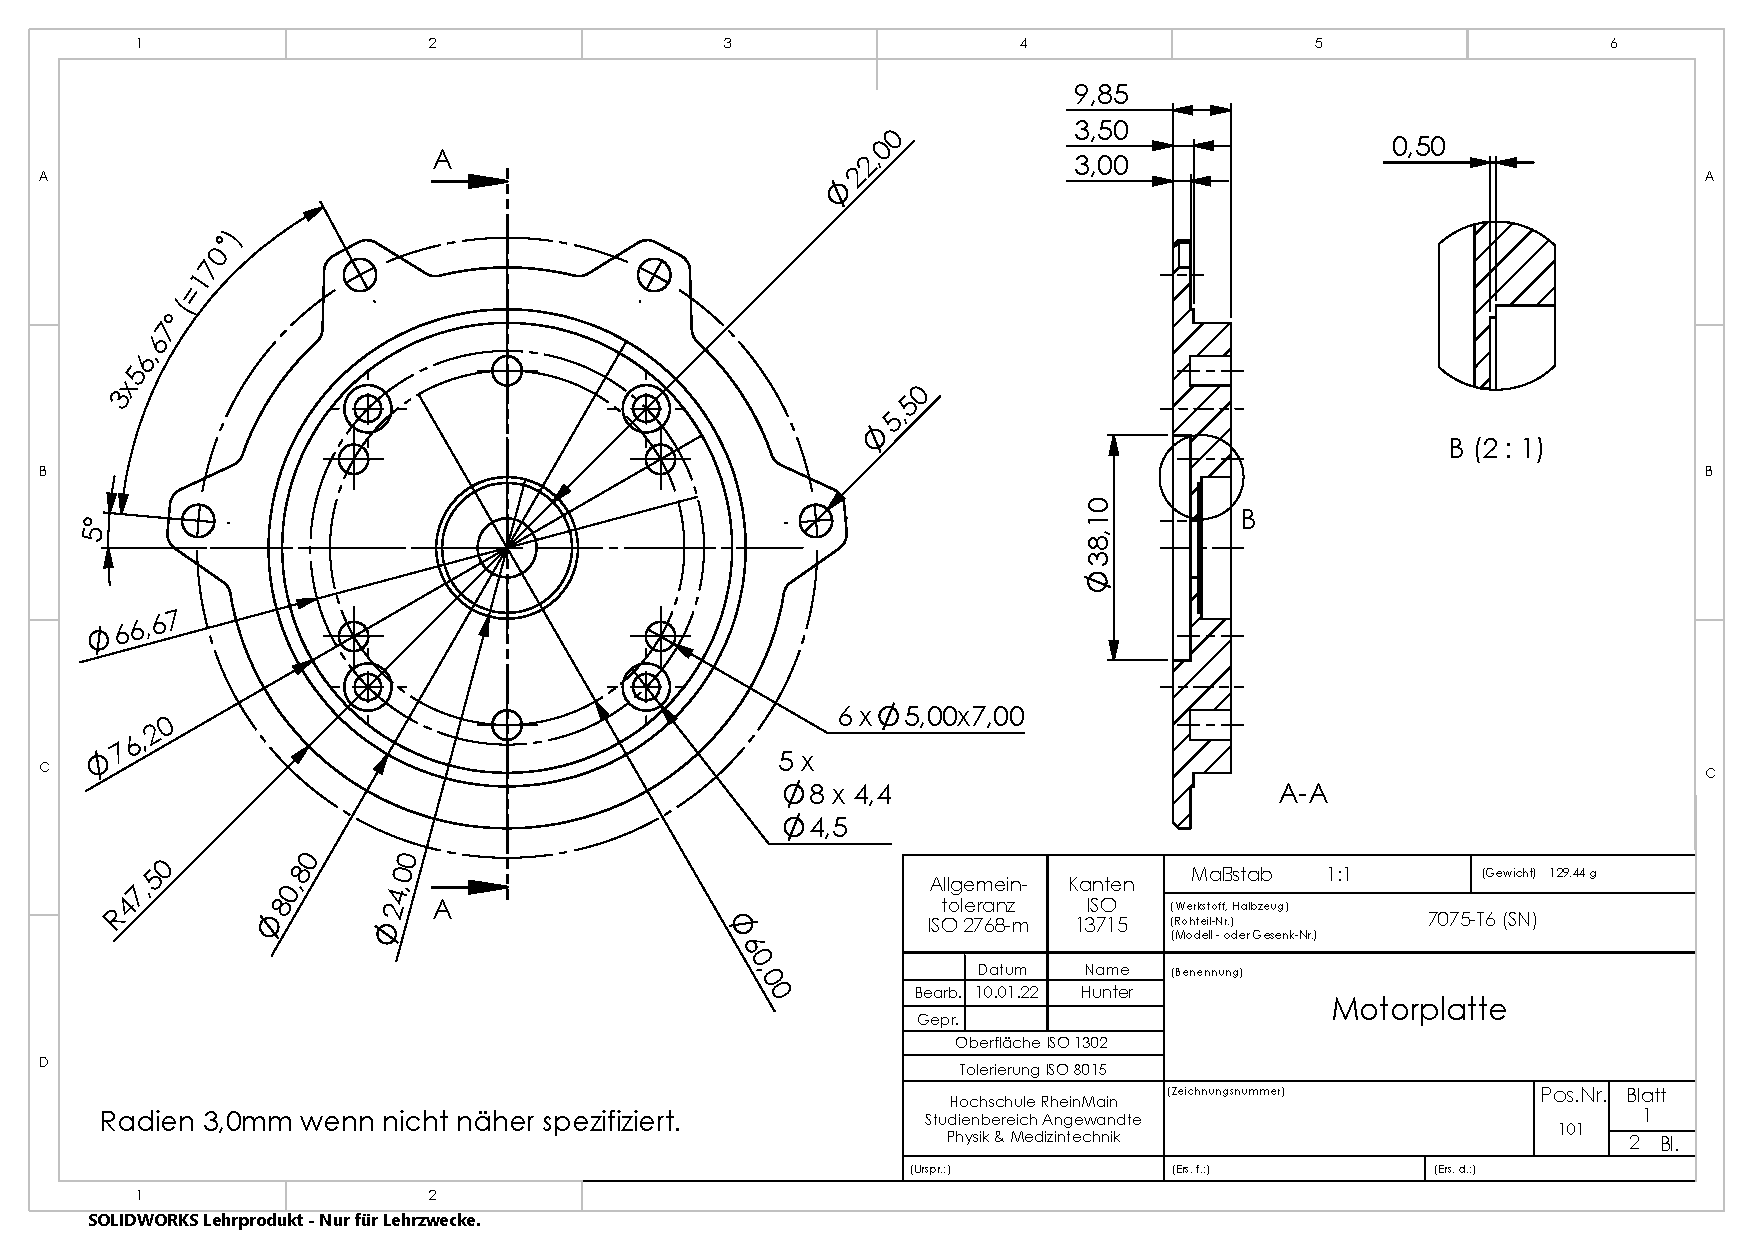
\includepdf[pages=-, angle=90, pagecommand={\thispagestyle{plain}}]{Abb/CAD/Drawings/Schulter/Motorplatte-Fixierplatte.pdf}
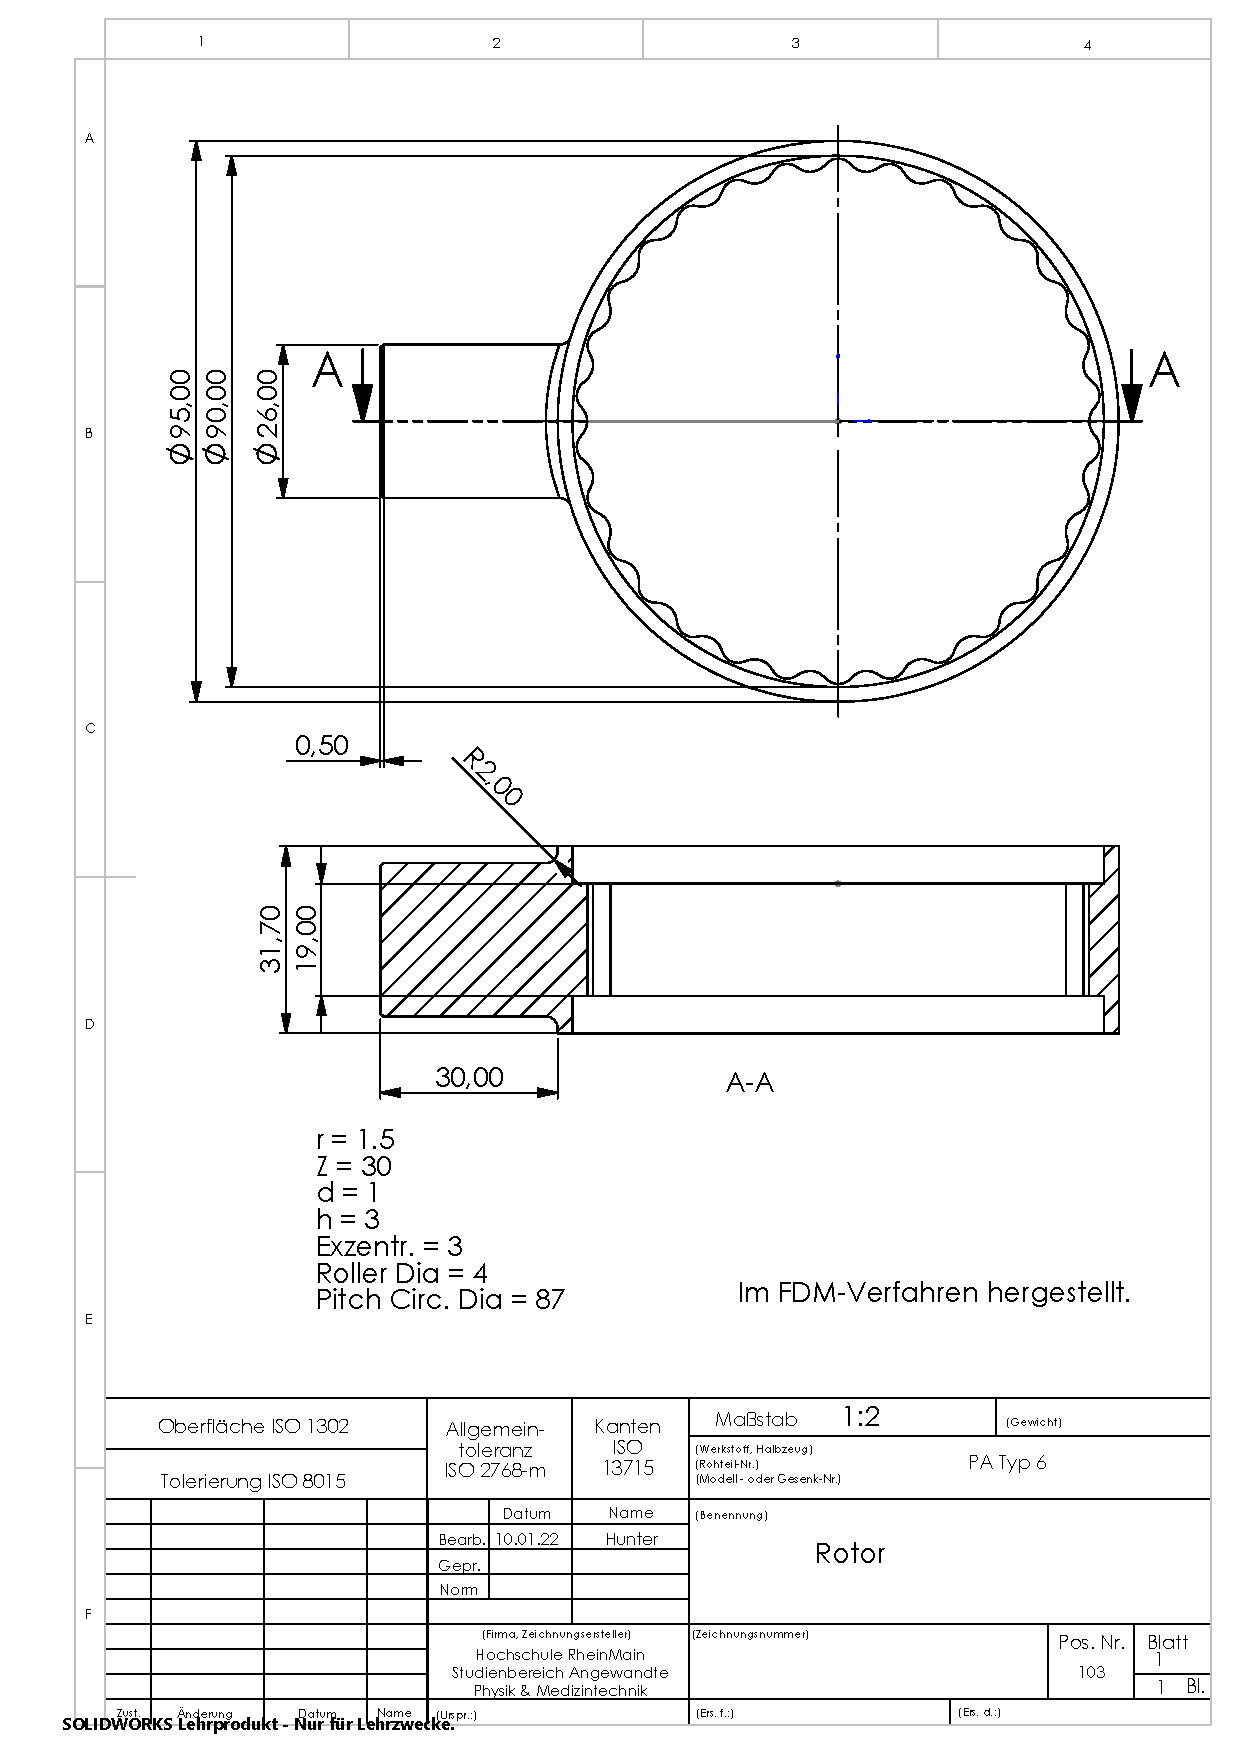
\includepdf[pages=-, angle=0, pagecommand={\thispagestyle{plain}}]{Abb/CAD/Drawings/Schulter/Rotor.pdf}
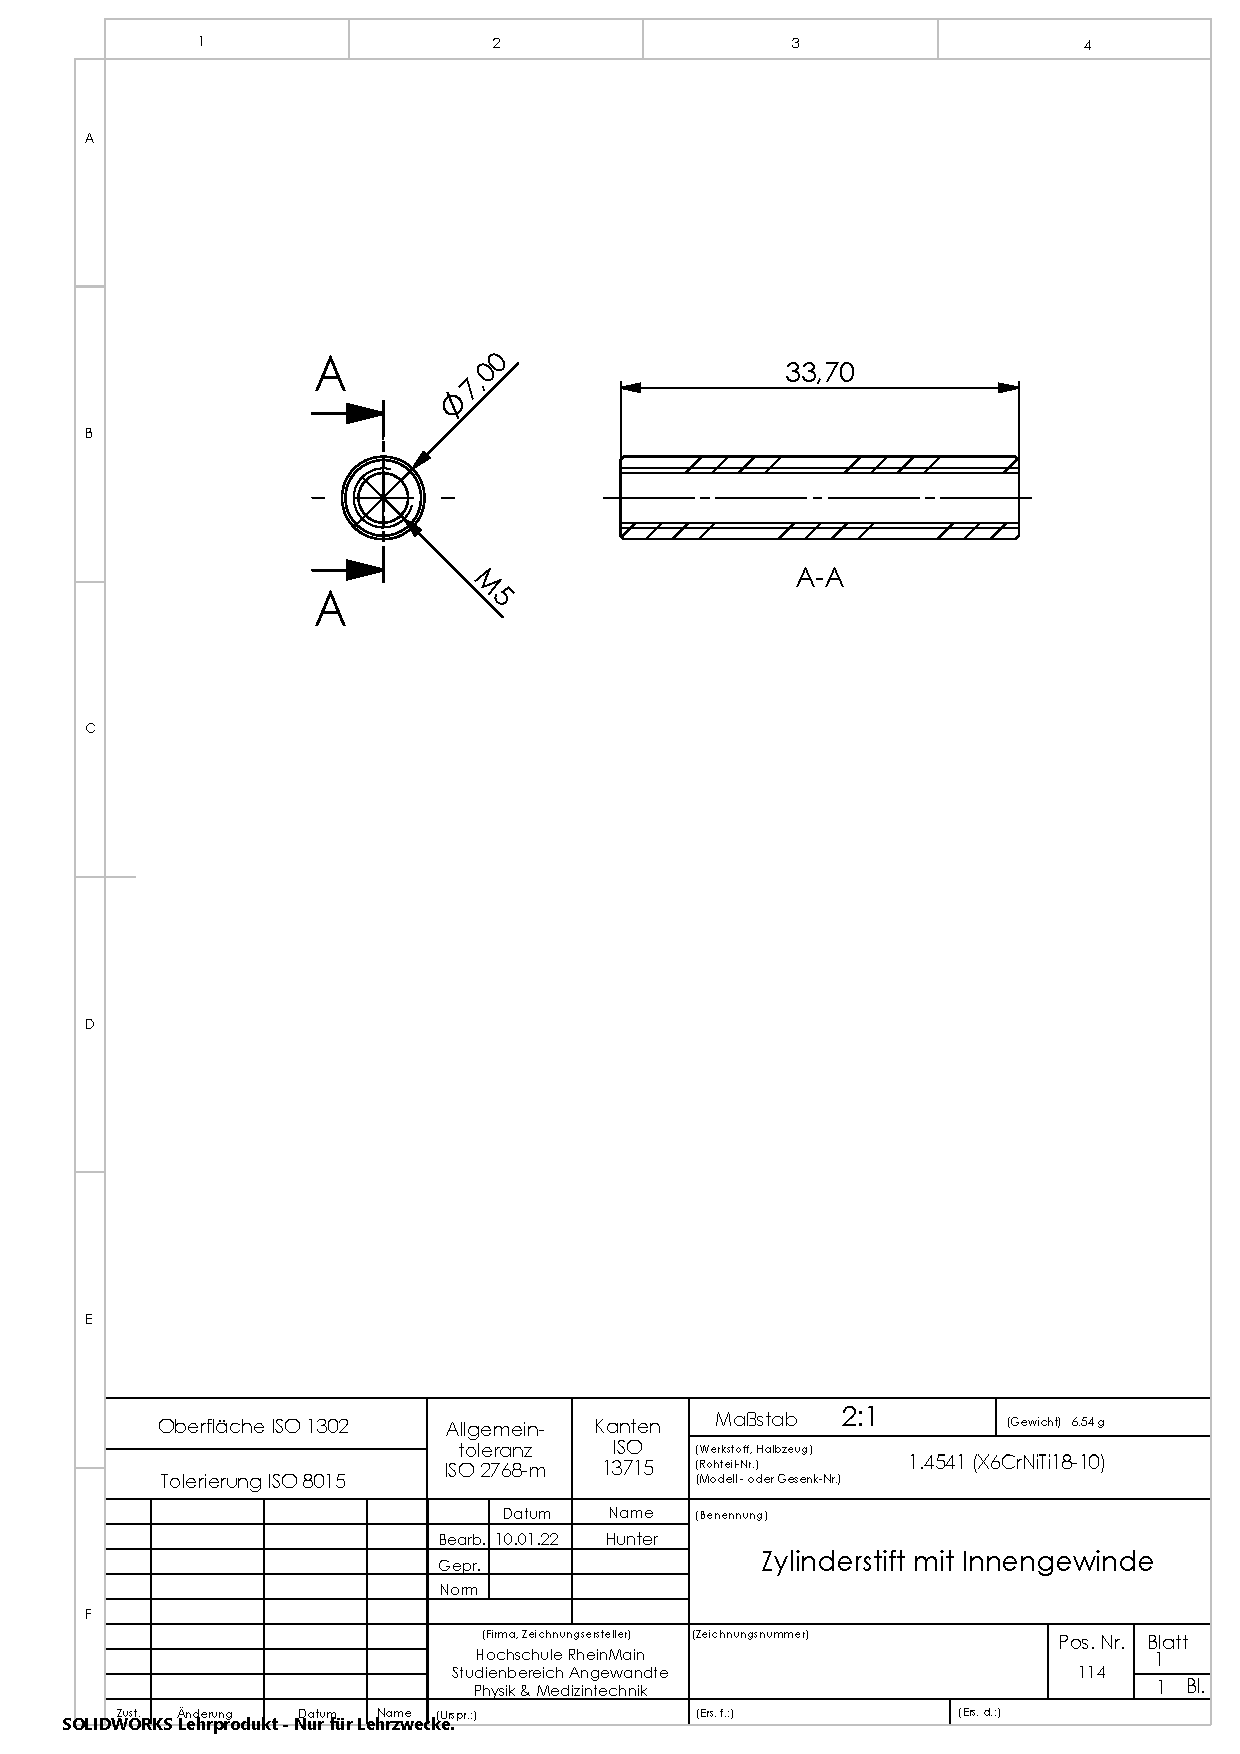
\includepdf[pages=-, angle=0, pagecommand={\thispagestyle{plain}}]{Abb/CAD/Drawings/Schulter/Zylinderstift-mit-Innengewinde.pdf}
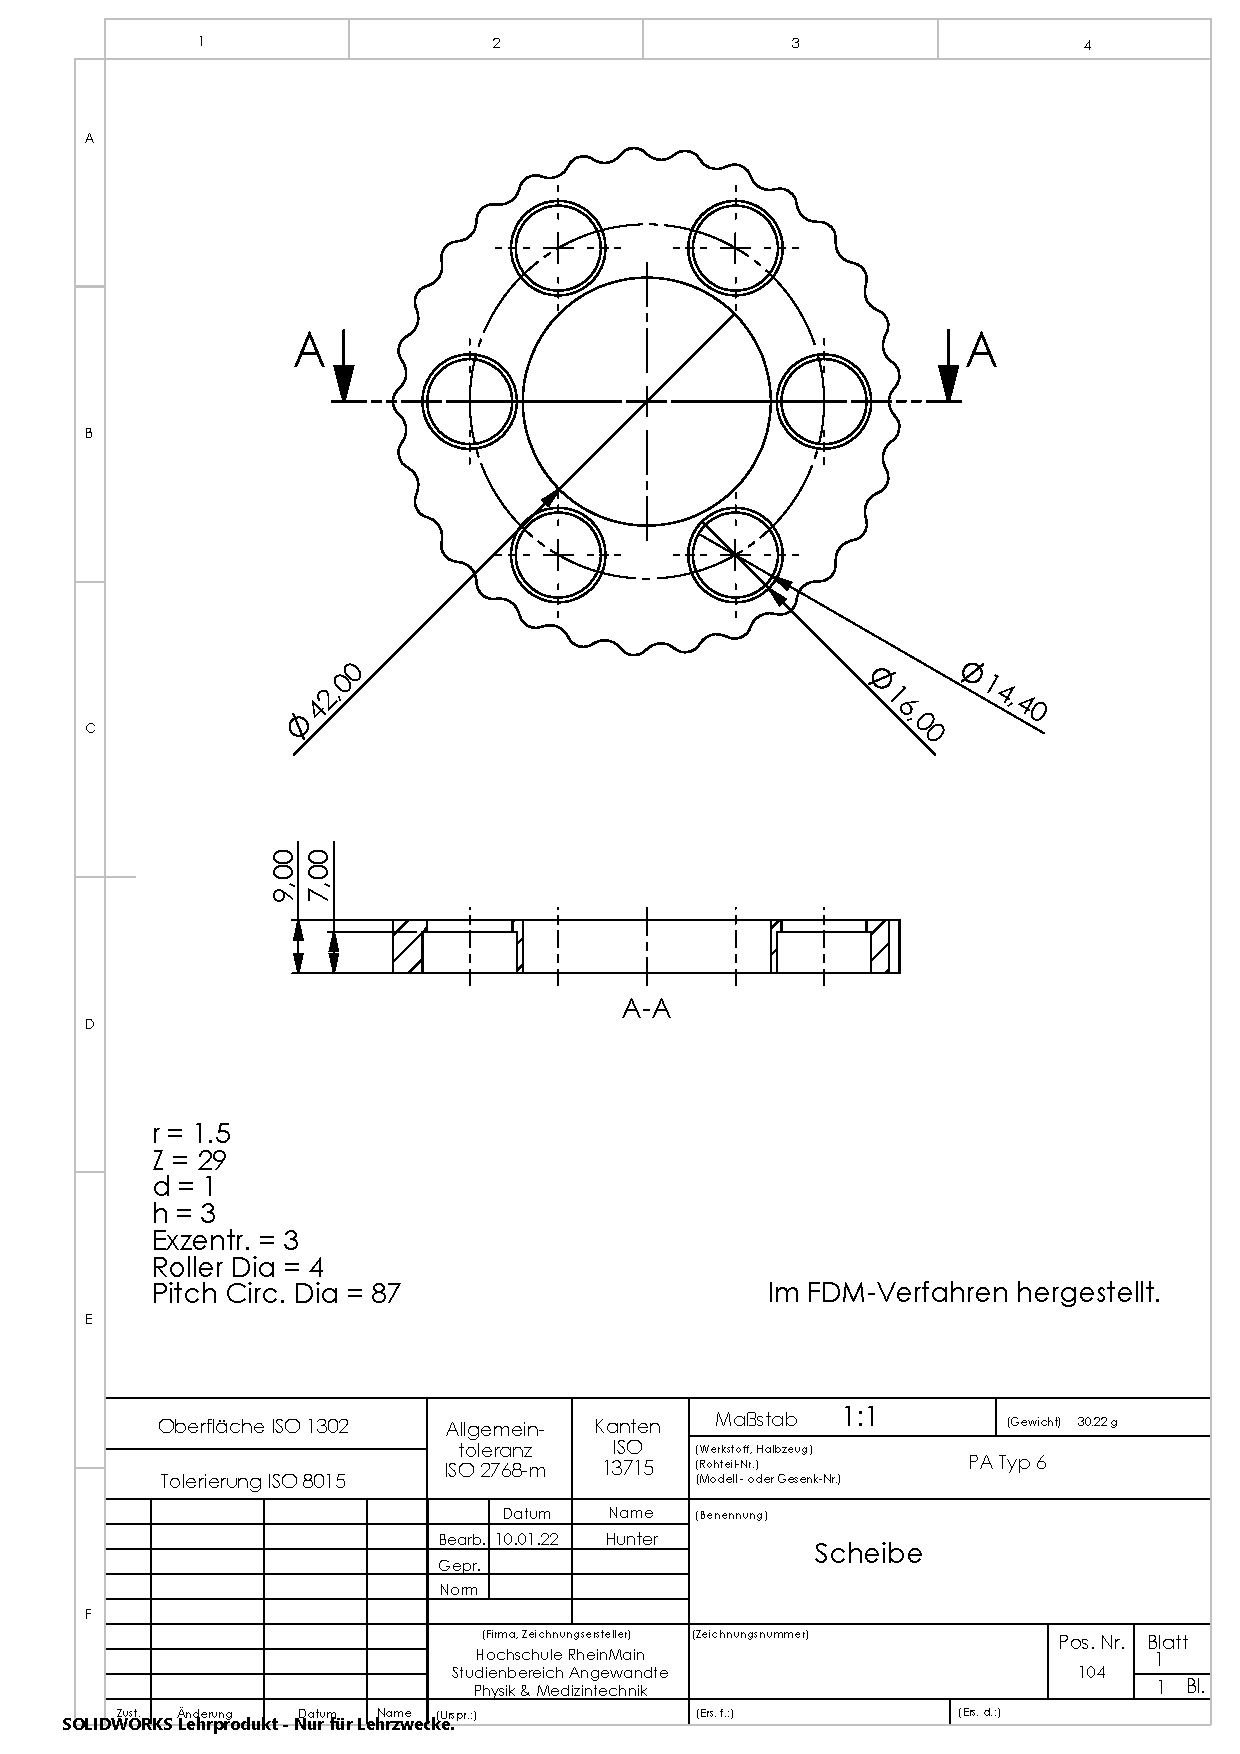
\includepdf[pages=-, angle=0, pagecommand={\thispagestyle{plain}}]{Abb/CAD/Drawings/Schulter/Scheibe.pdf}
%
\newpage
\setlength{\voffset}{-2.5 cm}
\setlength{\hoffset}{-2 cm}
\section{Einzelteilzeichnungen Arme}\label{sec:einzelteilzeichnungen arme}
\newpage
\setlength{\voffset}{0cm}
\setlength{\hoffset}{0cm}
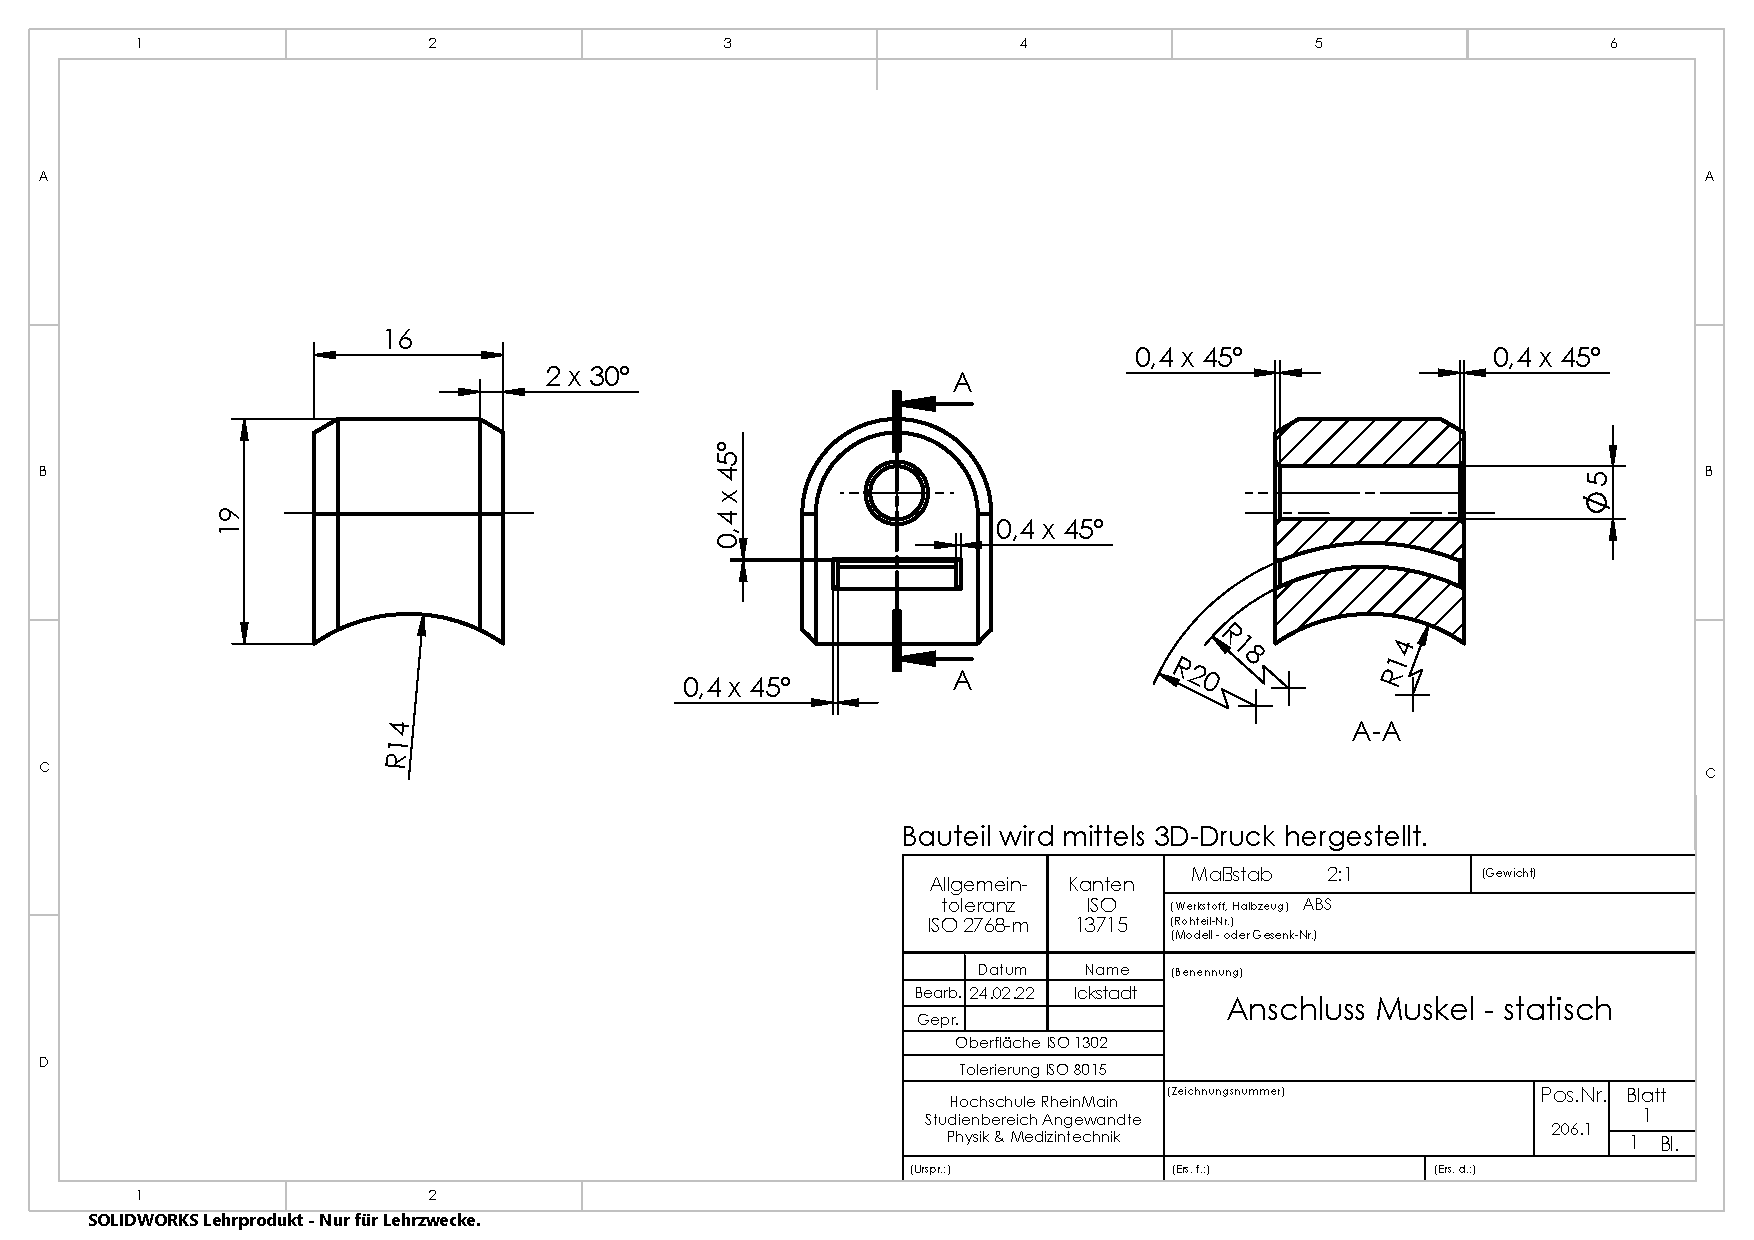
\includepdf[pages=-, angle=90, pagecommand={\thispagestyle{plain}}]{Abb/CAD/Drawings/Anschluss-Muskel-statisch.pdf}
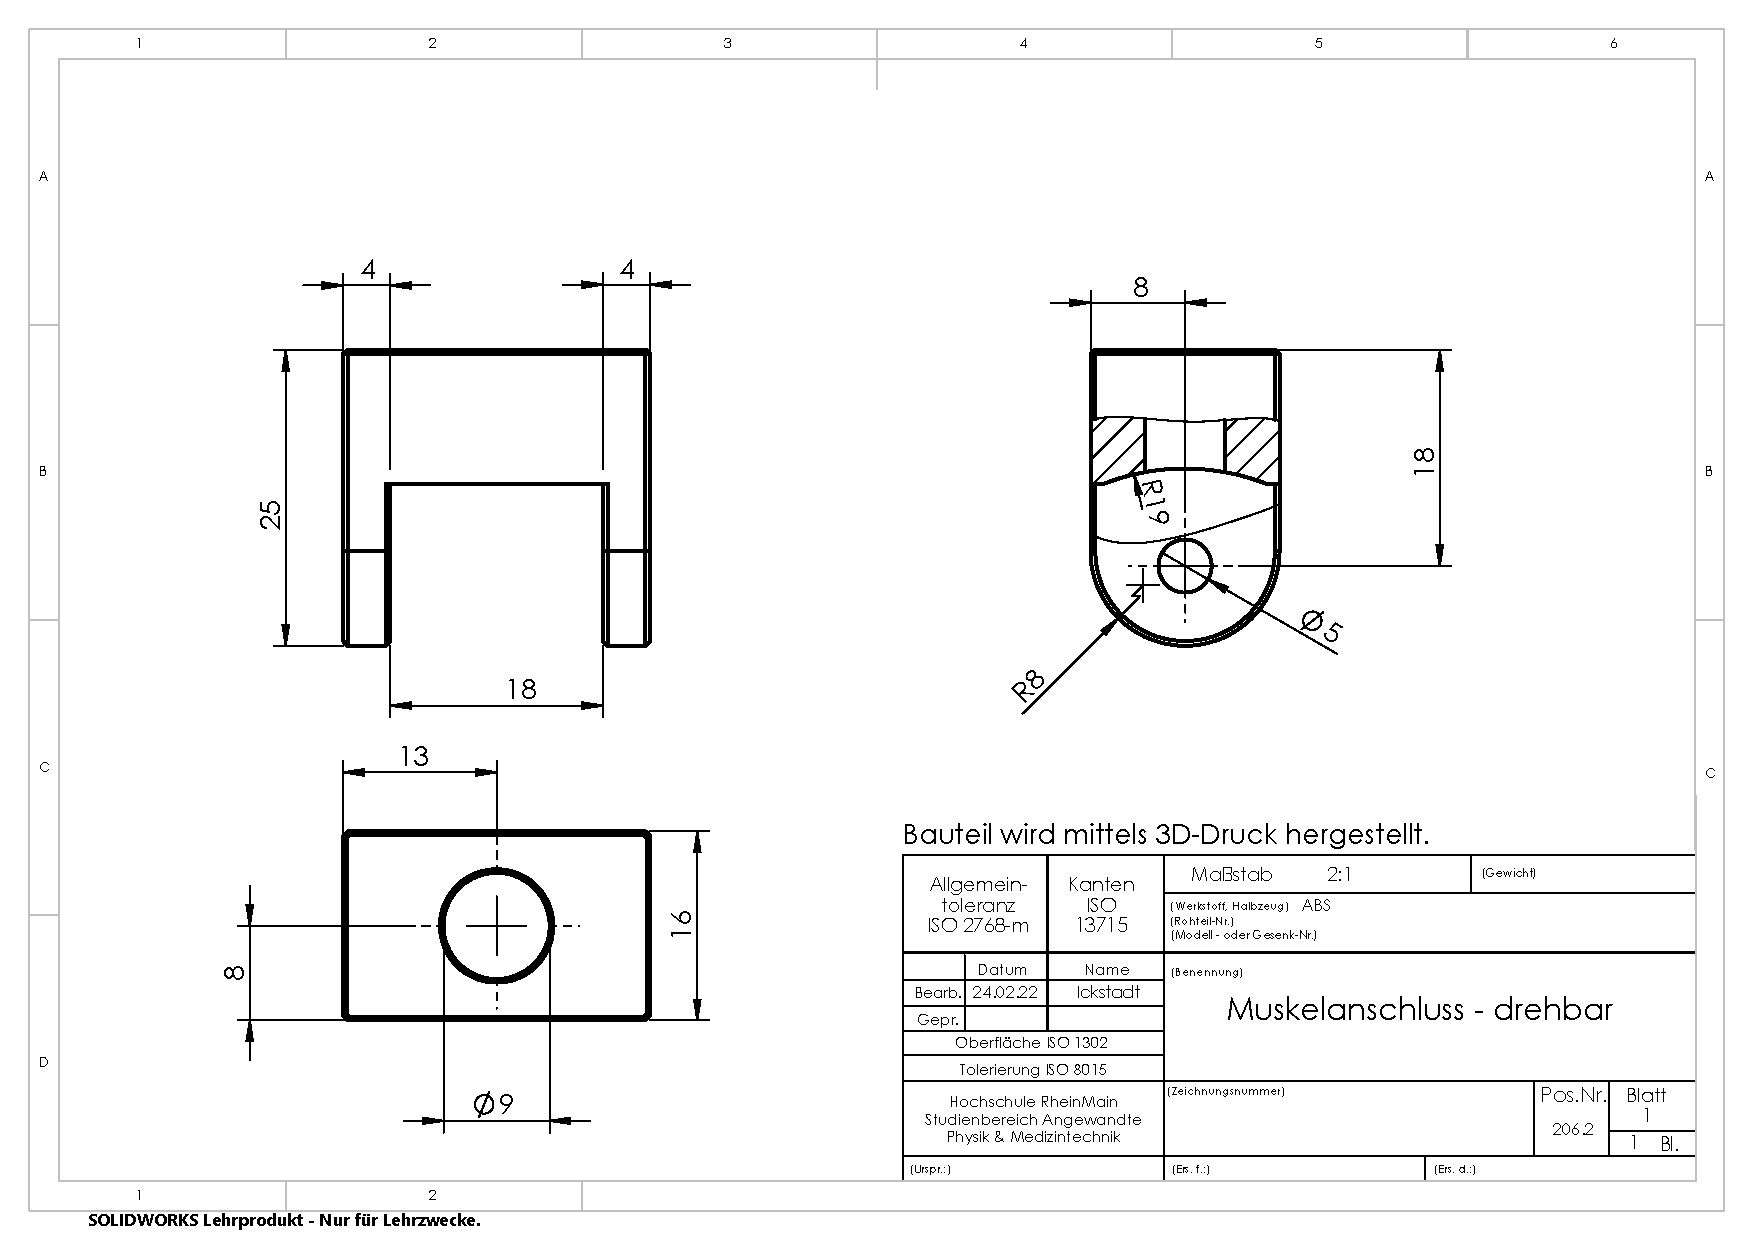
\includepdf[pages=-, angle=90, pagecommand={\thispagestyle{plain}}]{Abb/CAD/Drawings/Muskelanschluss-drehbar.pdf}
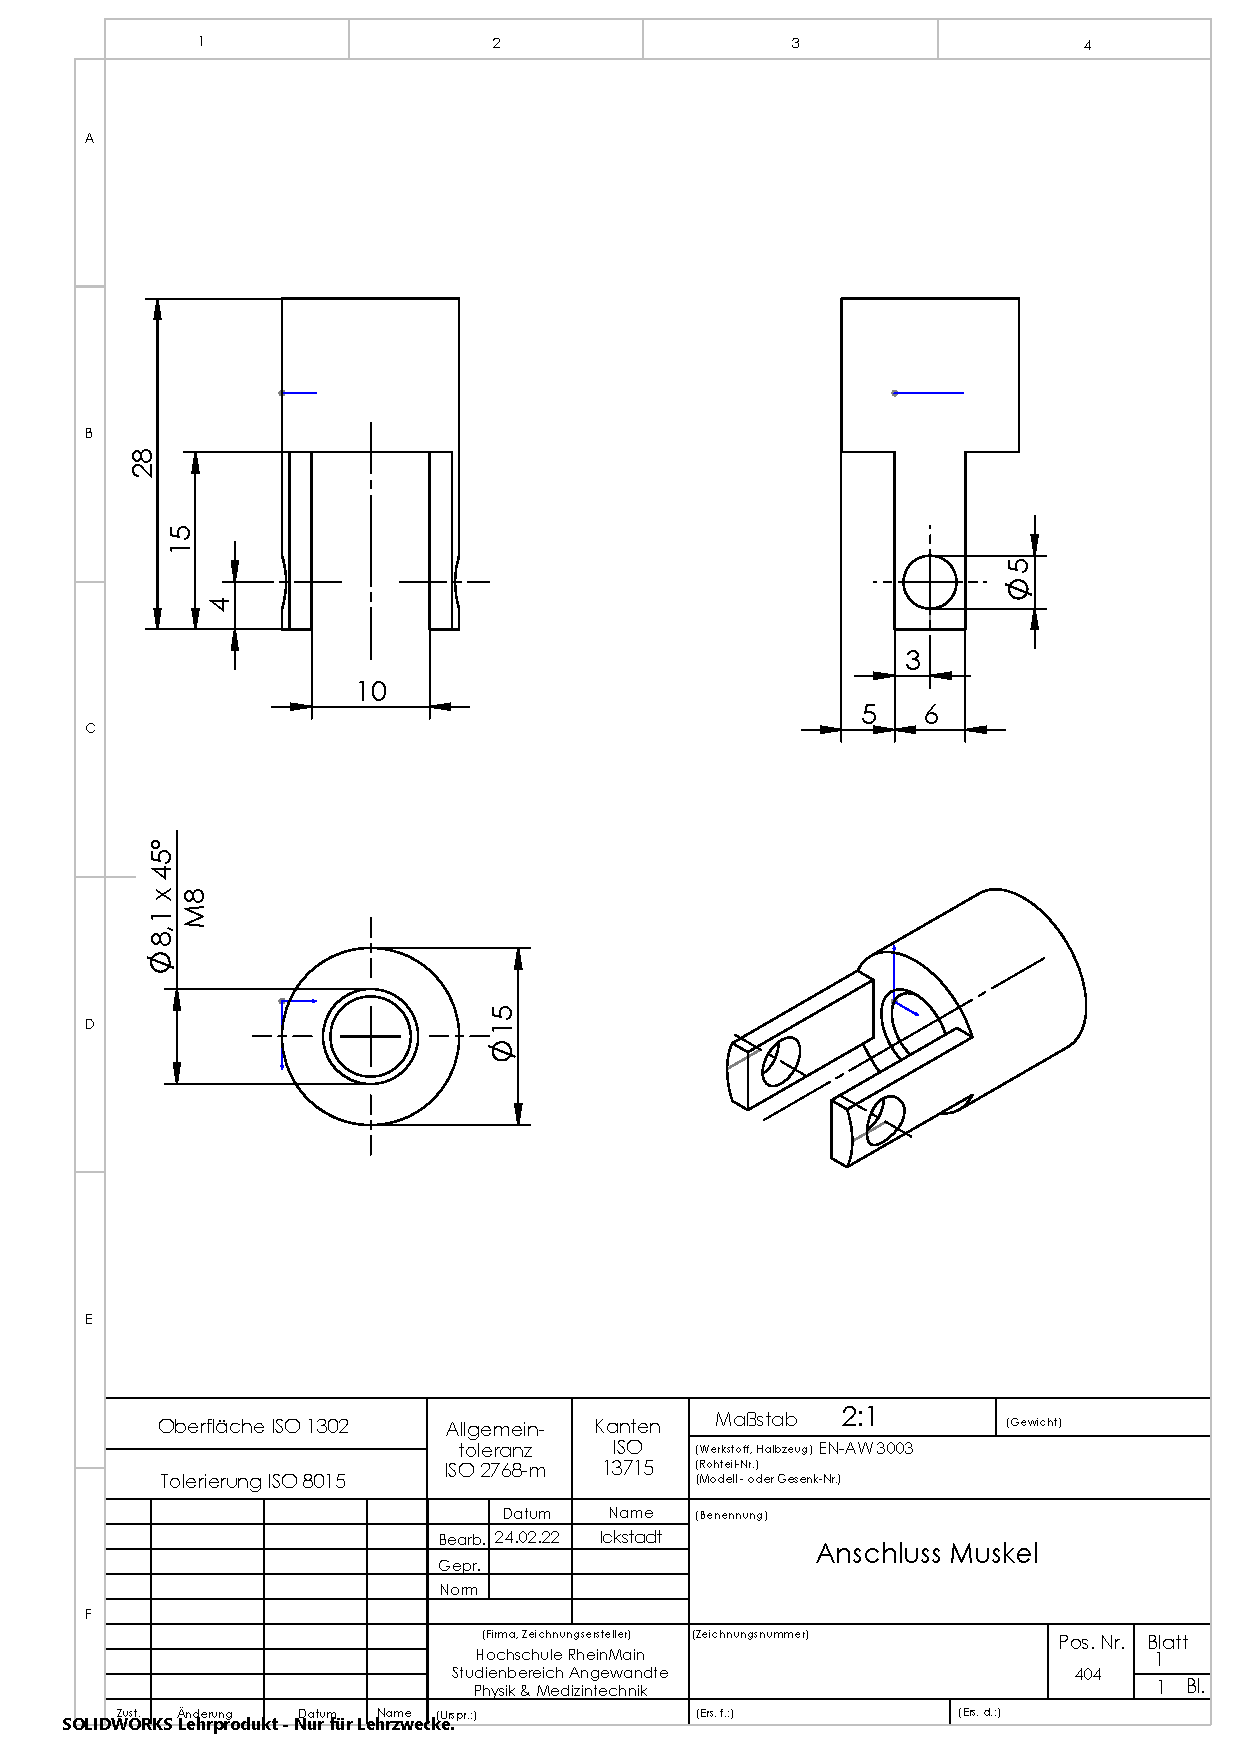
\includepdf[pages=-, angle=0, pagecommand={\thispagestyle{plain}}]{Abb/CAD/Drawings/Anschluss-Muskel.pdf}
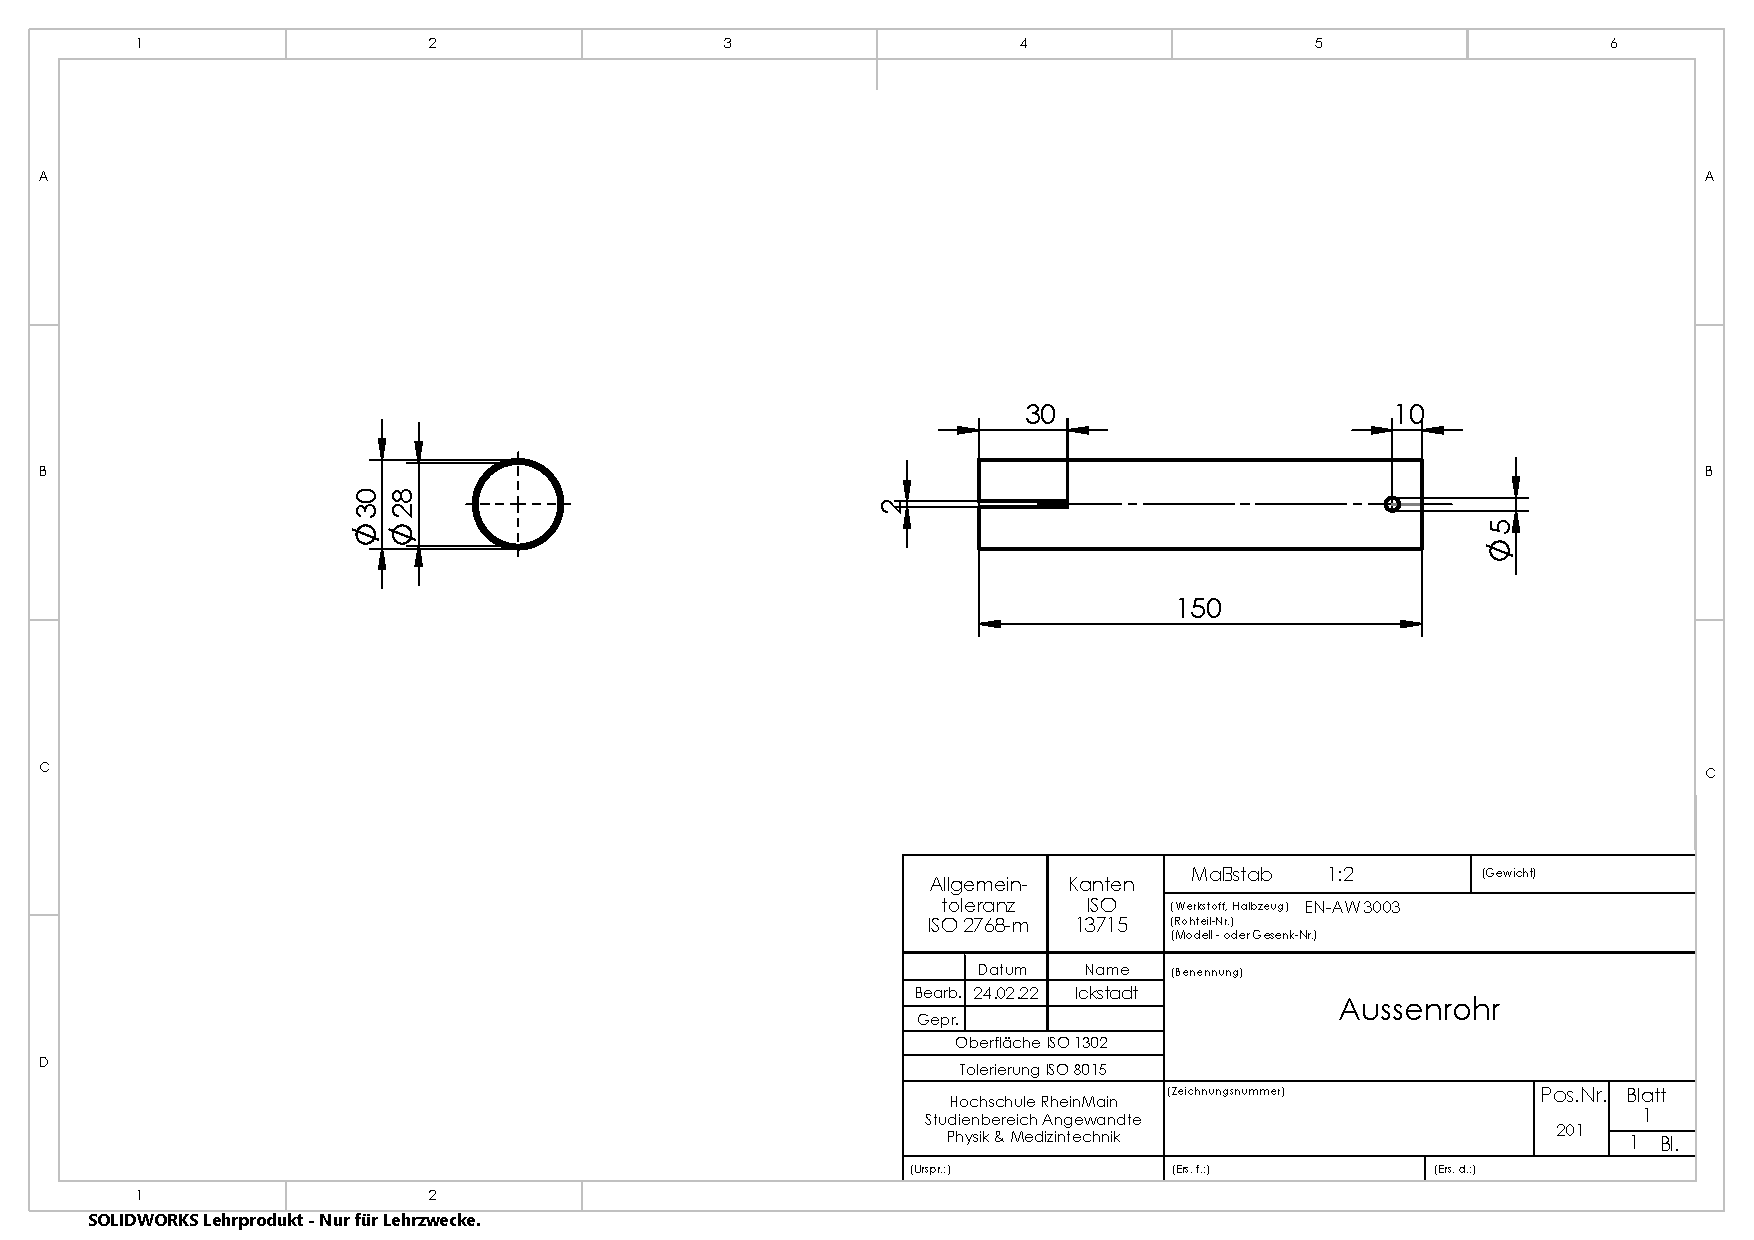
\includepdf[pages=-, angle=90, pagecommand={\thispagestyle{plain}}]{Abb/CAD/Drawings/Aussenrohr.pdf}
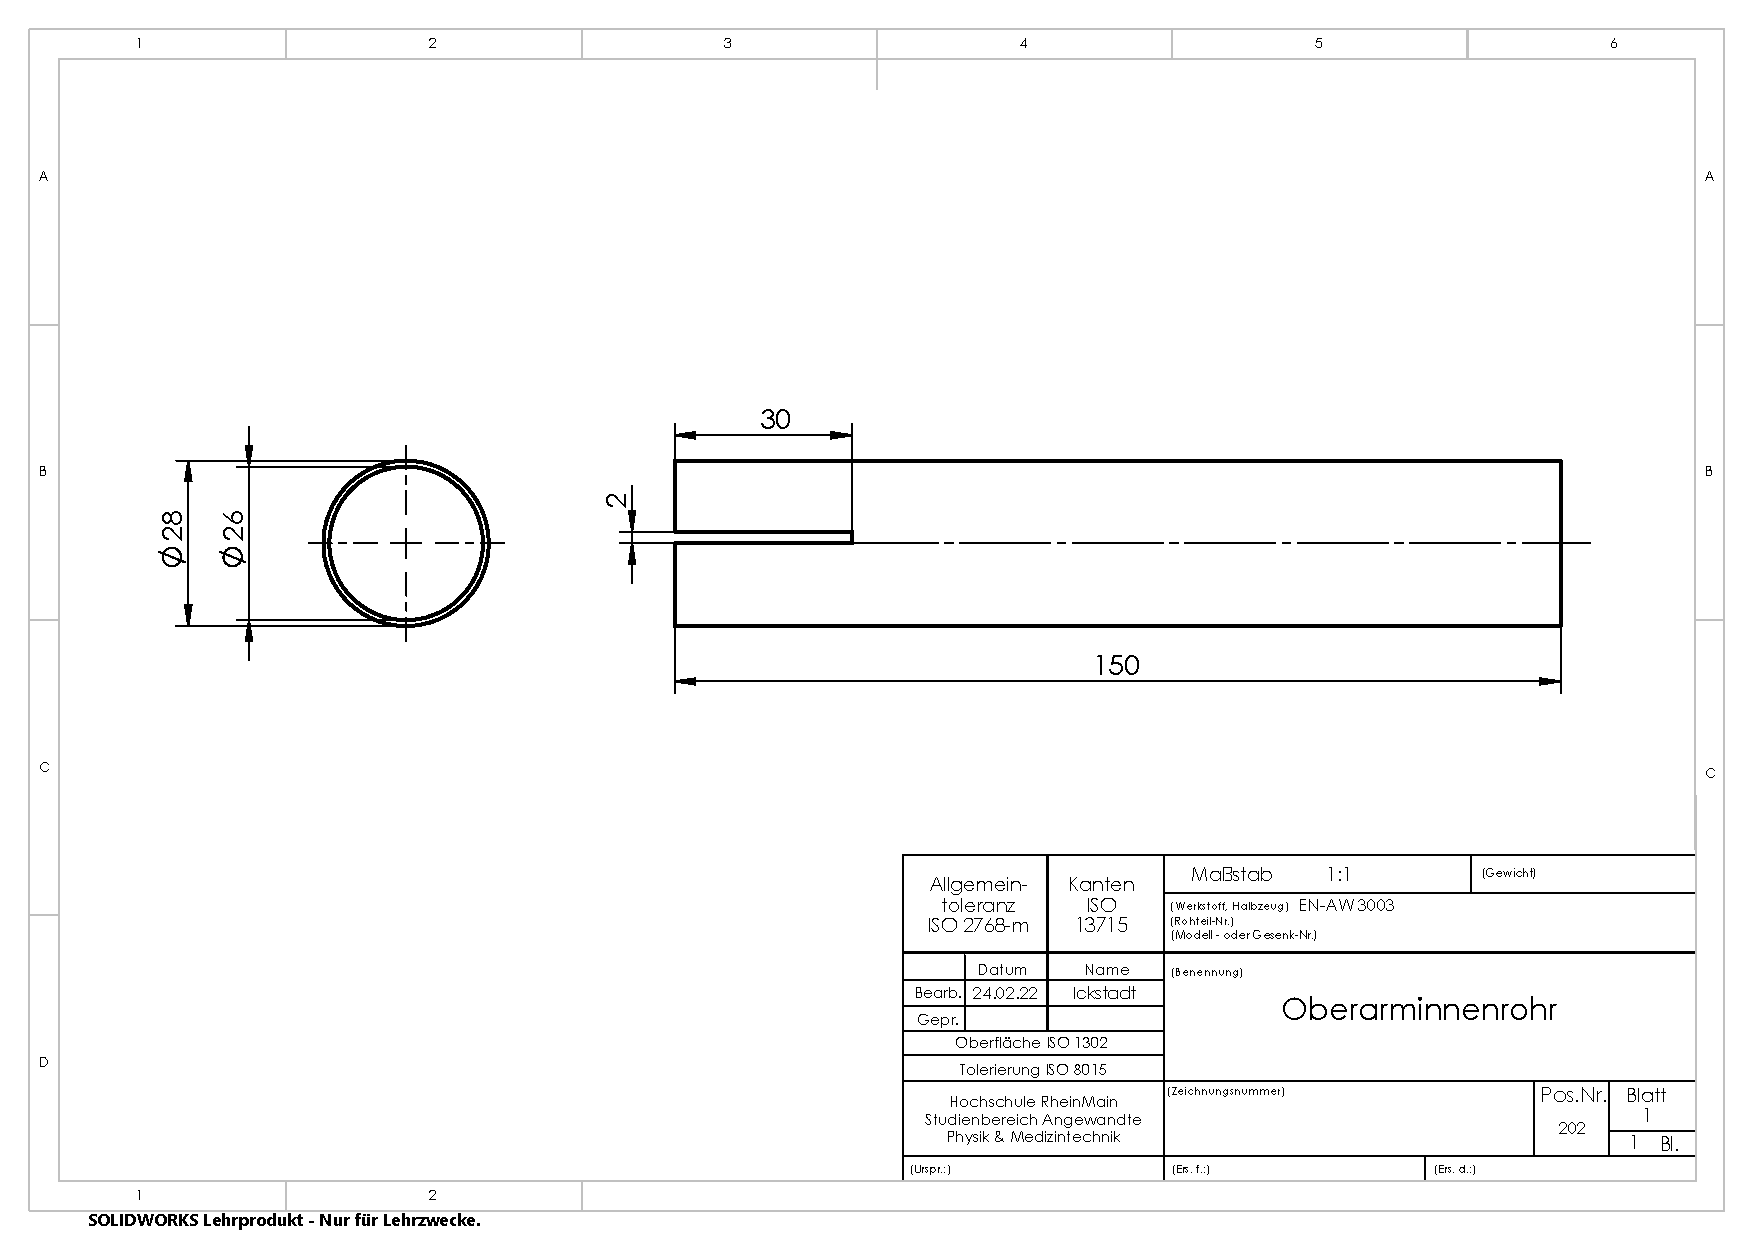
\includepdf[pages=-, angle=90, pagecommand={\thispagestyle{plain}}]{Abb/CAD/Drawings/Oberarminnenrohr.pdf}
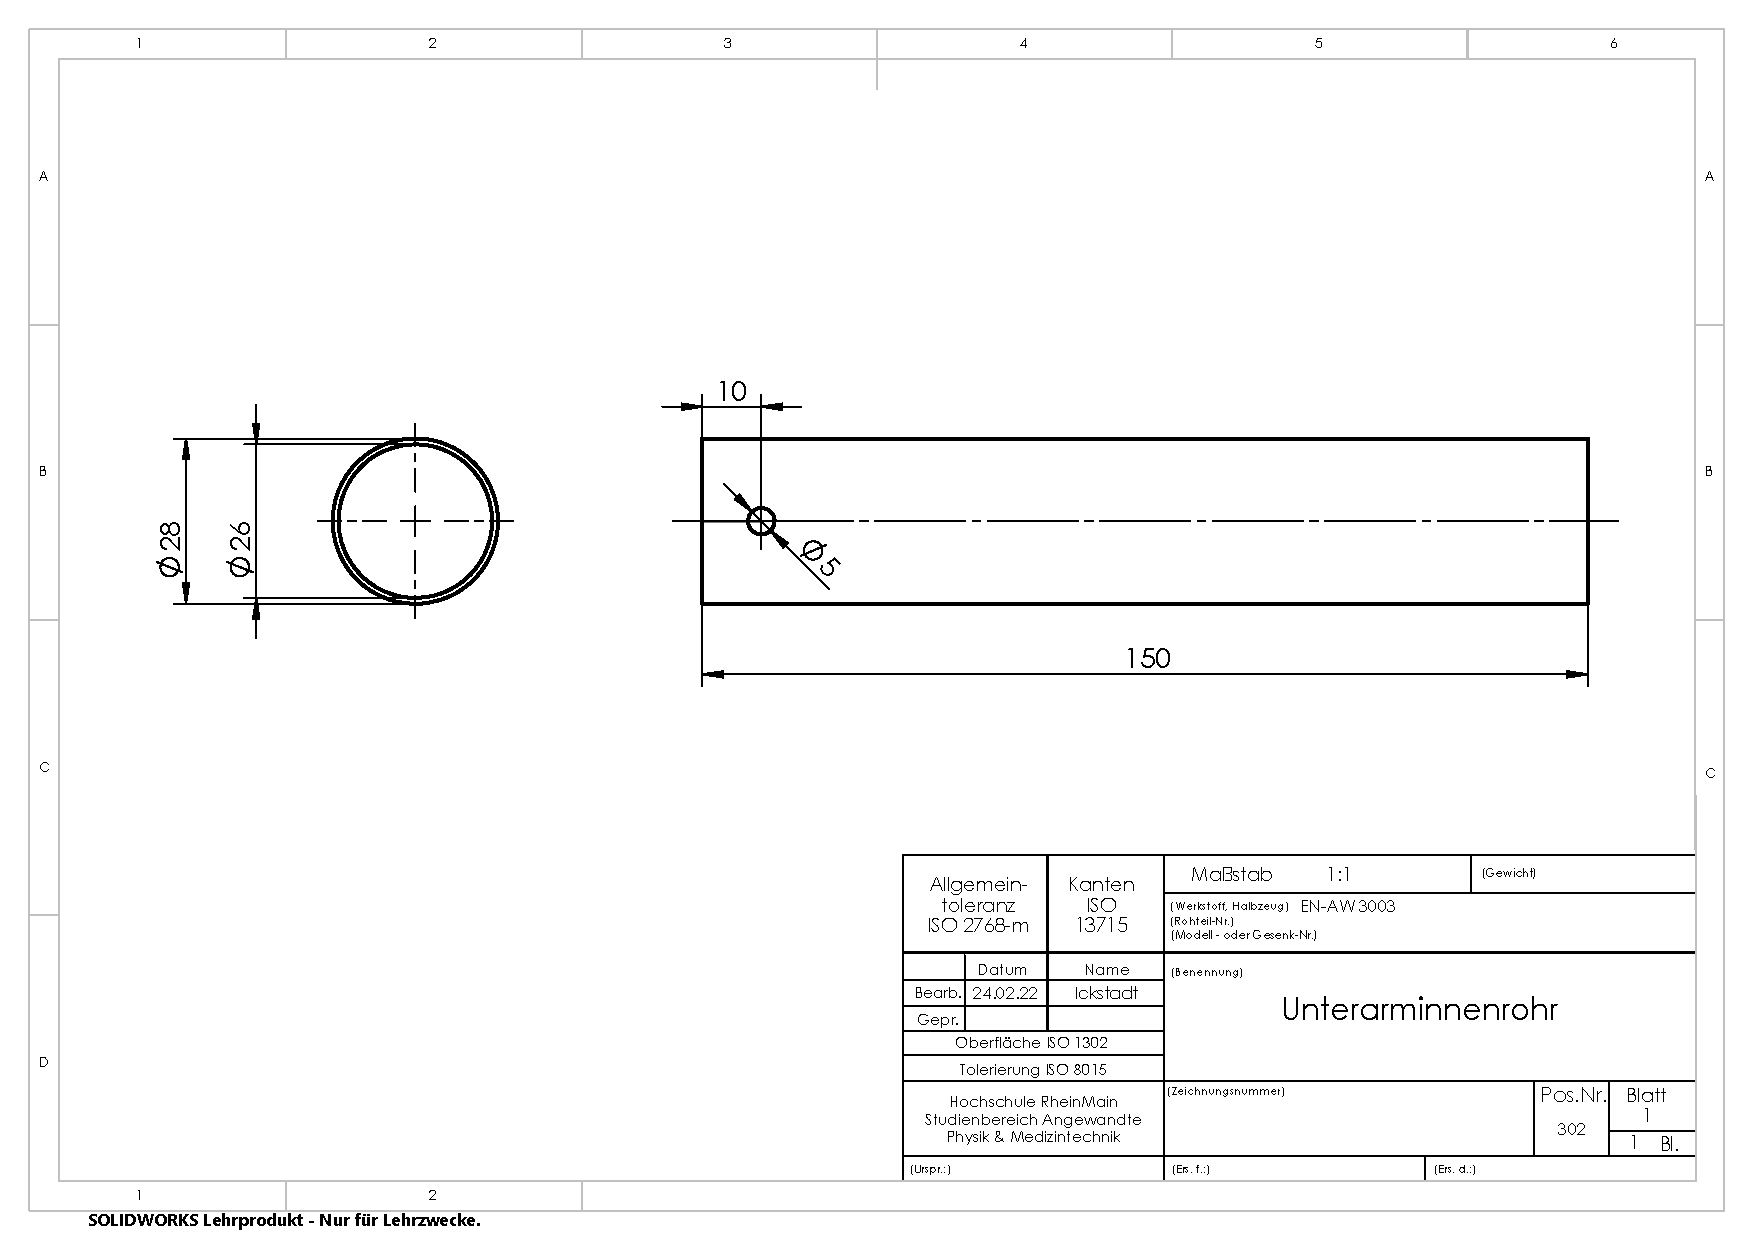
\includepdf[pages=-, angle=90, pagecommand={\thispagestyle{plain}}]{Abb/CAD/Drawings/Unterarminnenrohr.pdf}
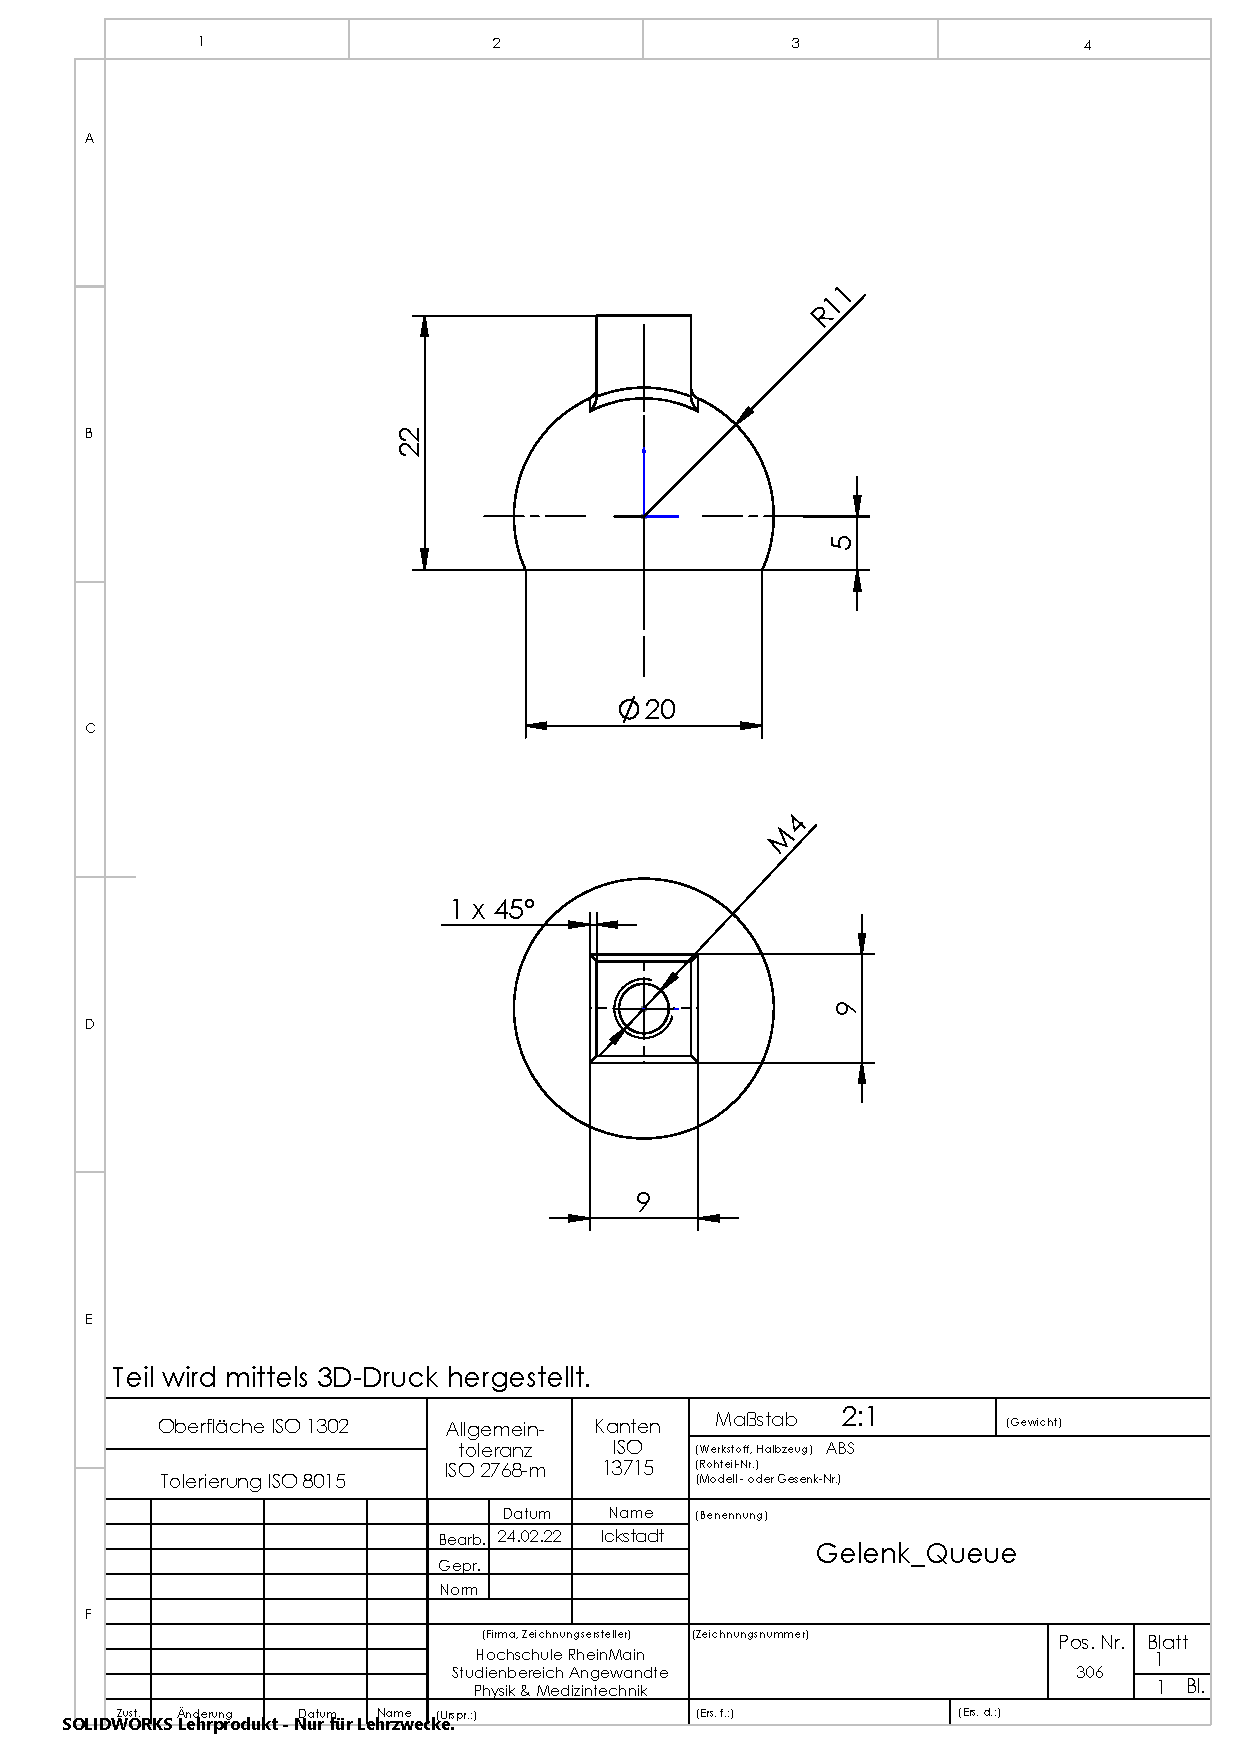
\includepdf[pages=-, angle=0, pagecommand={\thispagestyle{plain}}]{Abb/CAD/Drawings/Gelenk-Queue.pdf}
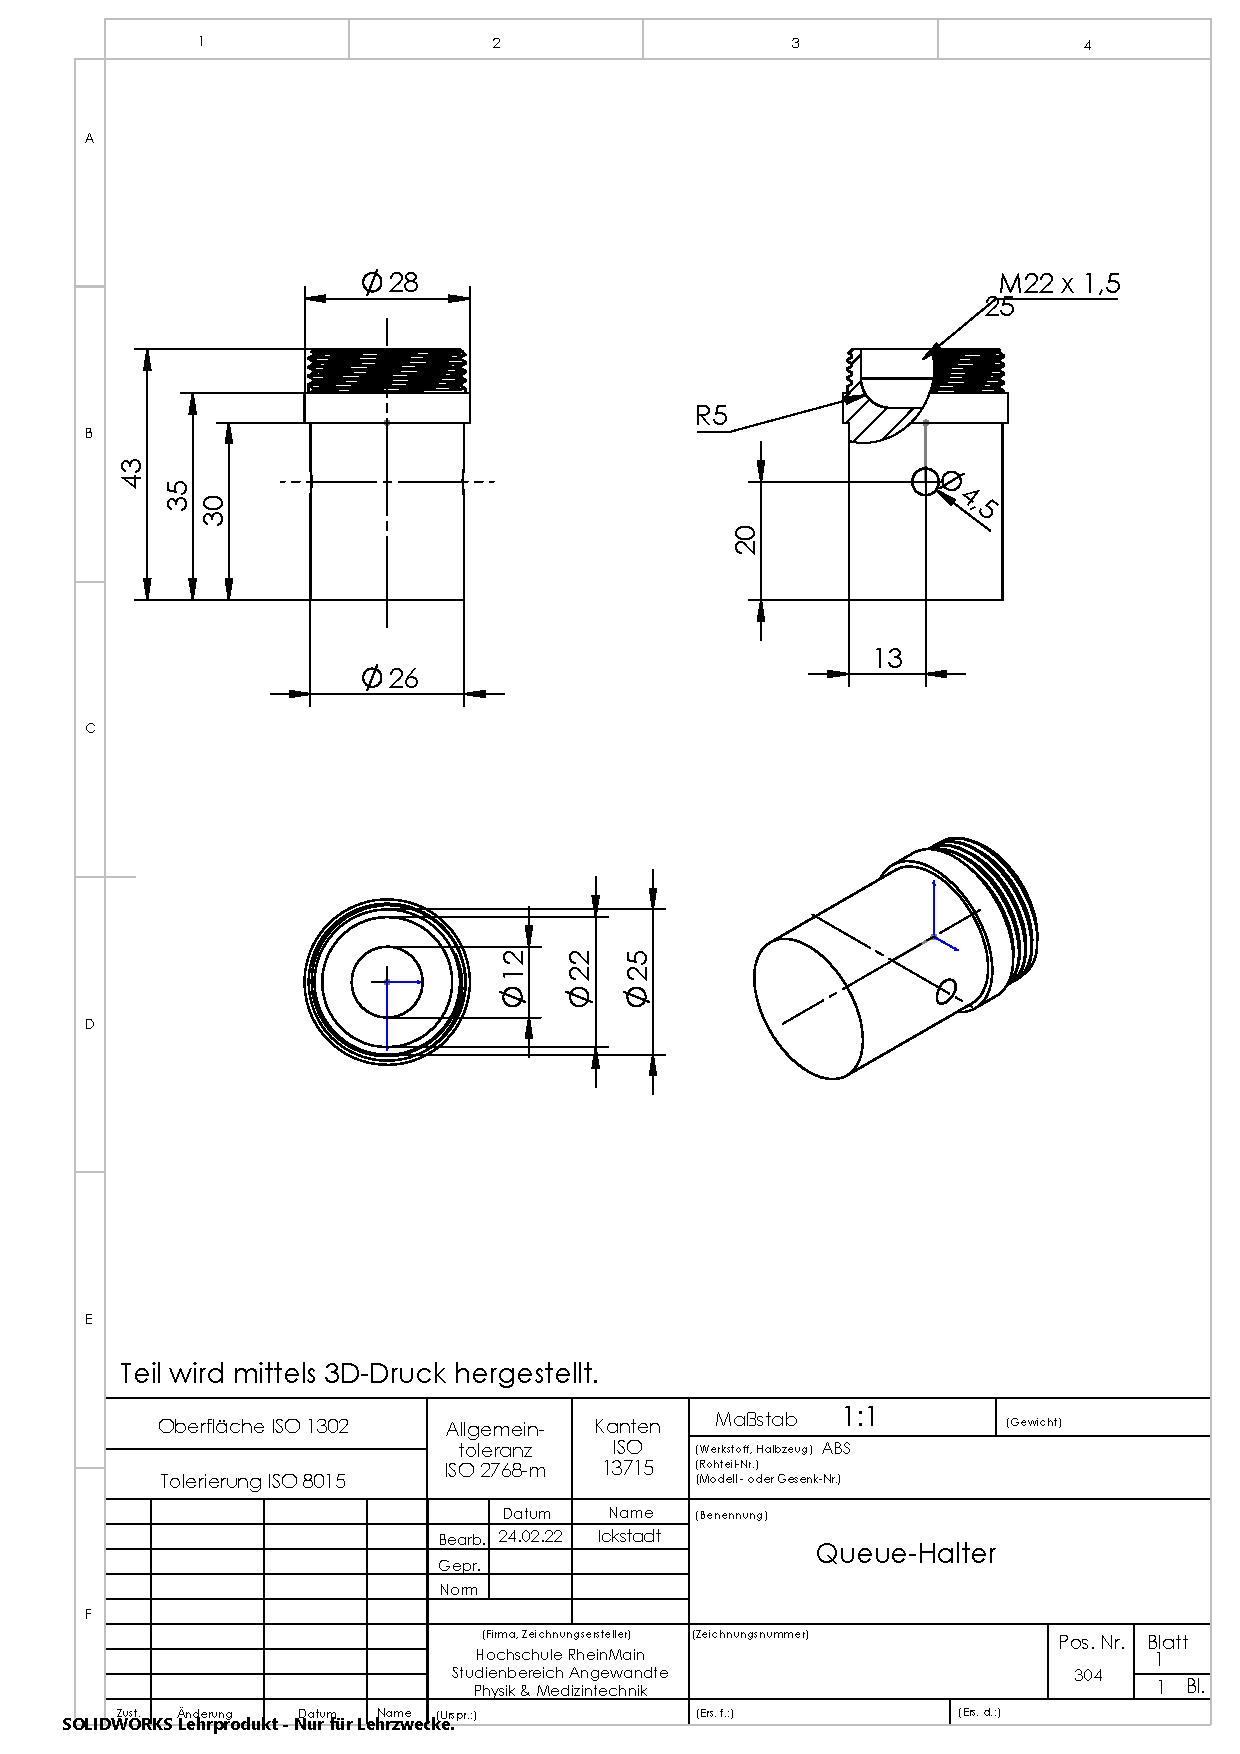
\includepdf[pages=-, angle=0, pagecommand={\thispagestyle{plain}}]{Abb/CAD/Drawings/Queue-Halter.pdf}
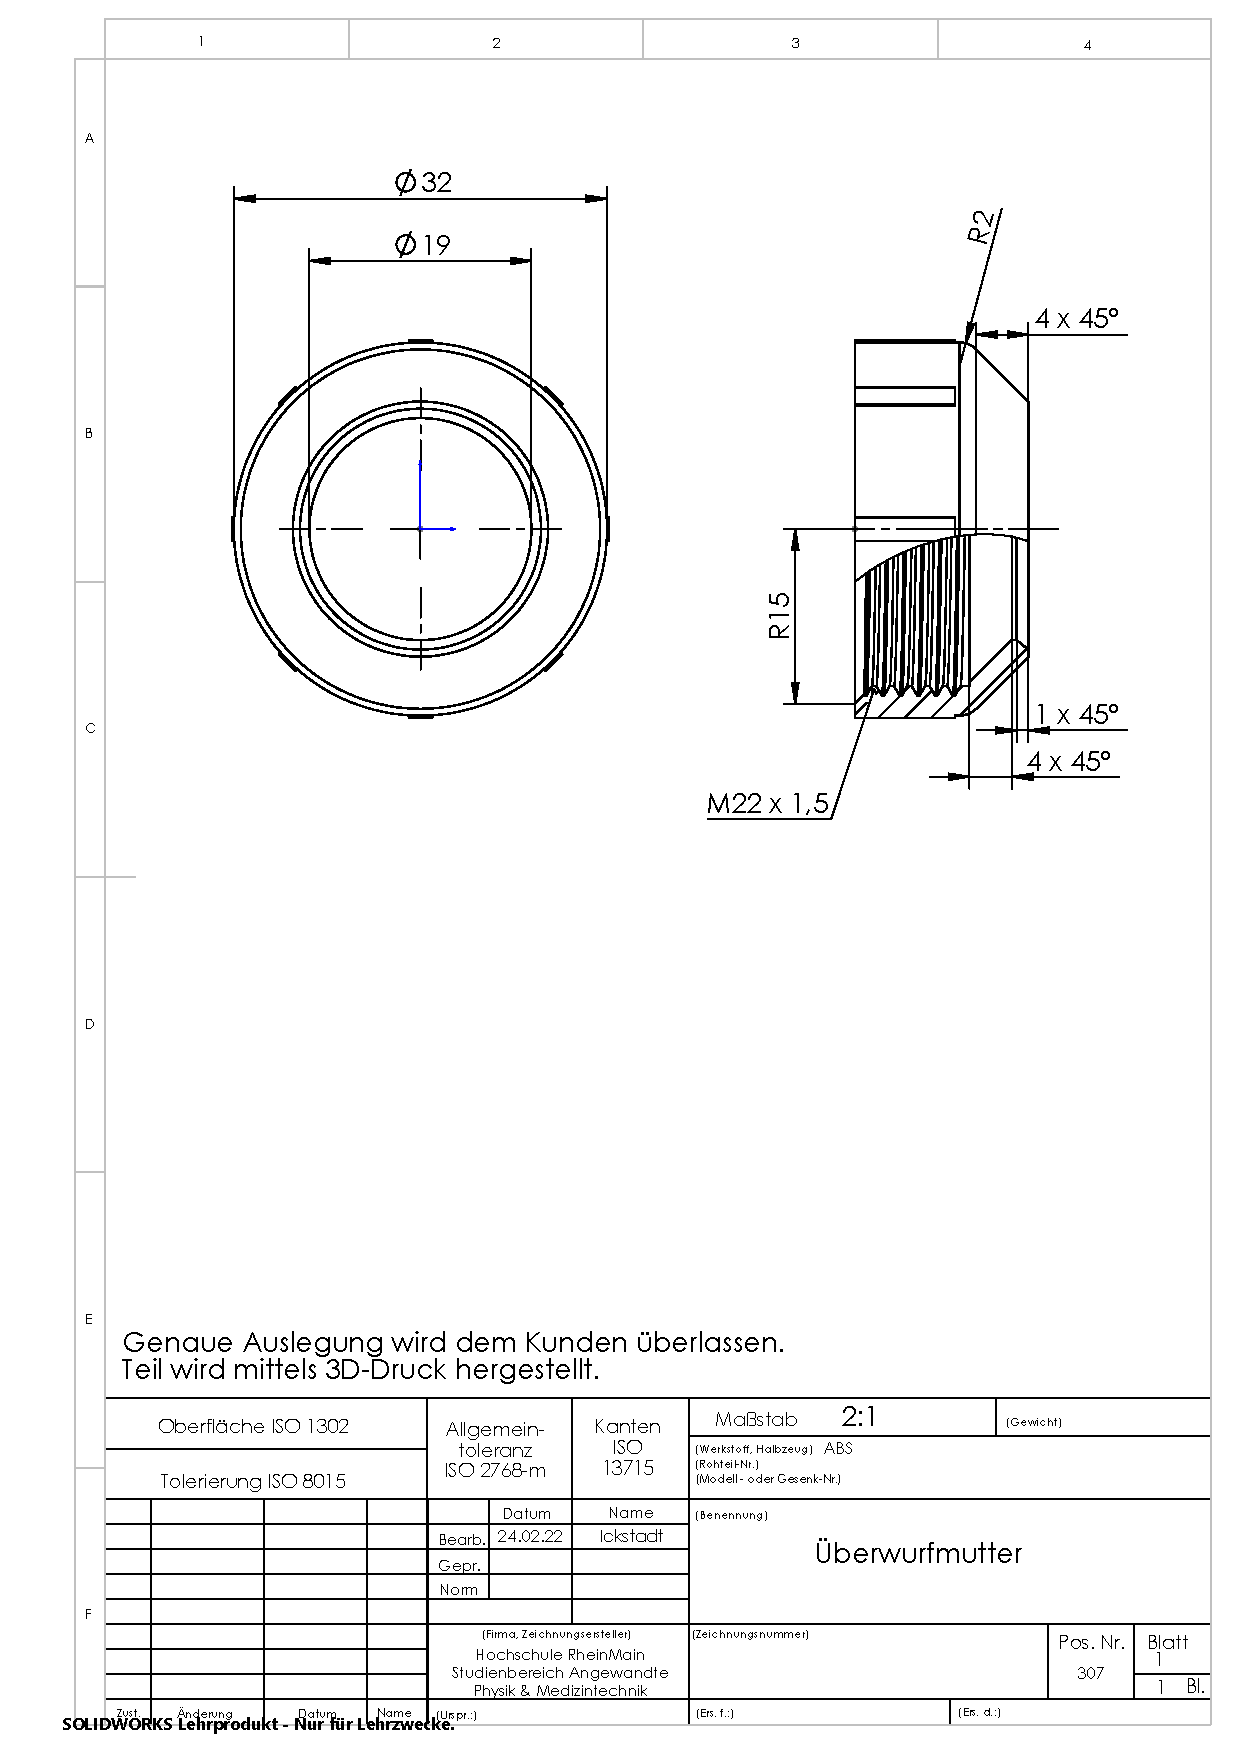
\includepdf[pages=-, angle=0, pagecommand={\thispagestyle{plain}}]{Abb/CAD/Drawings/Ueberwurfmutter.pdf}
%
\newpage
\setlength{\voffset}{-2.5 cm}
\setlength{\hoffset}{-2 cm}
\section{Einzelteilzeichnungen Ellbogengelenk}\label{sec:einzelteilzeichnungen ellbogengelenk}
\newpage
\setlength{\voffset}{0cm}
\setlength{\hoffset}{0cm}
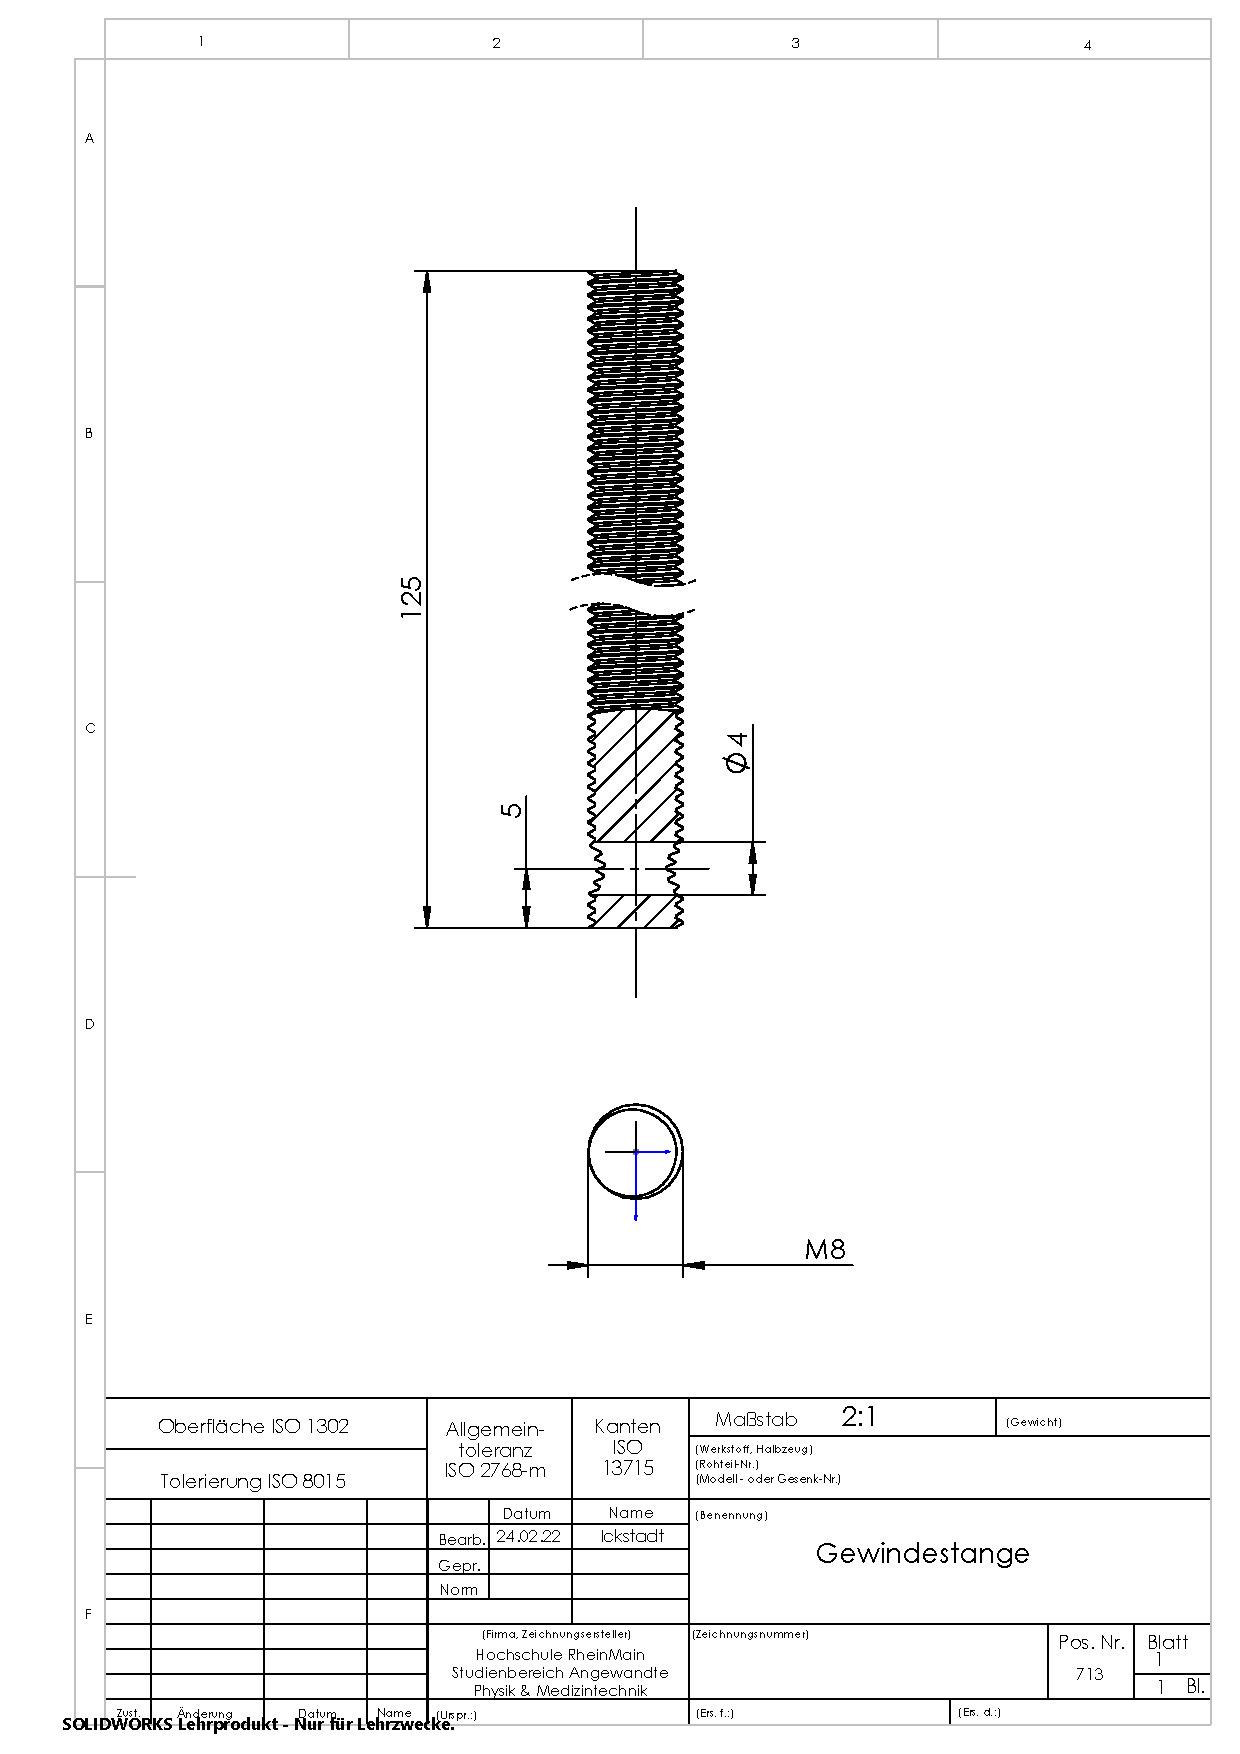
\includepdf[pages=-, angle=0, pagecommand={\thispagestyle{plain}}]{Abb/CAD/Drawings/Gewindestange.pdf}
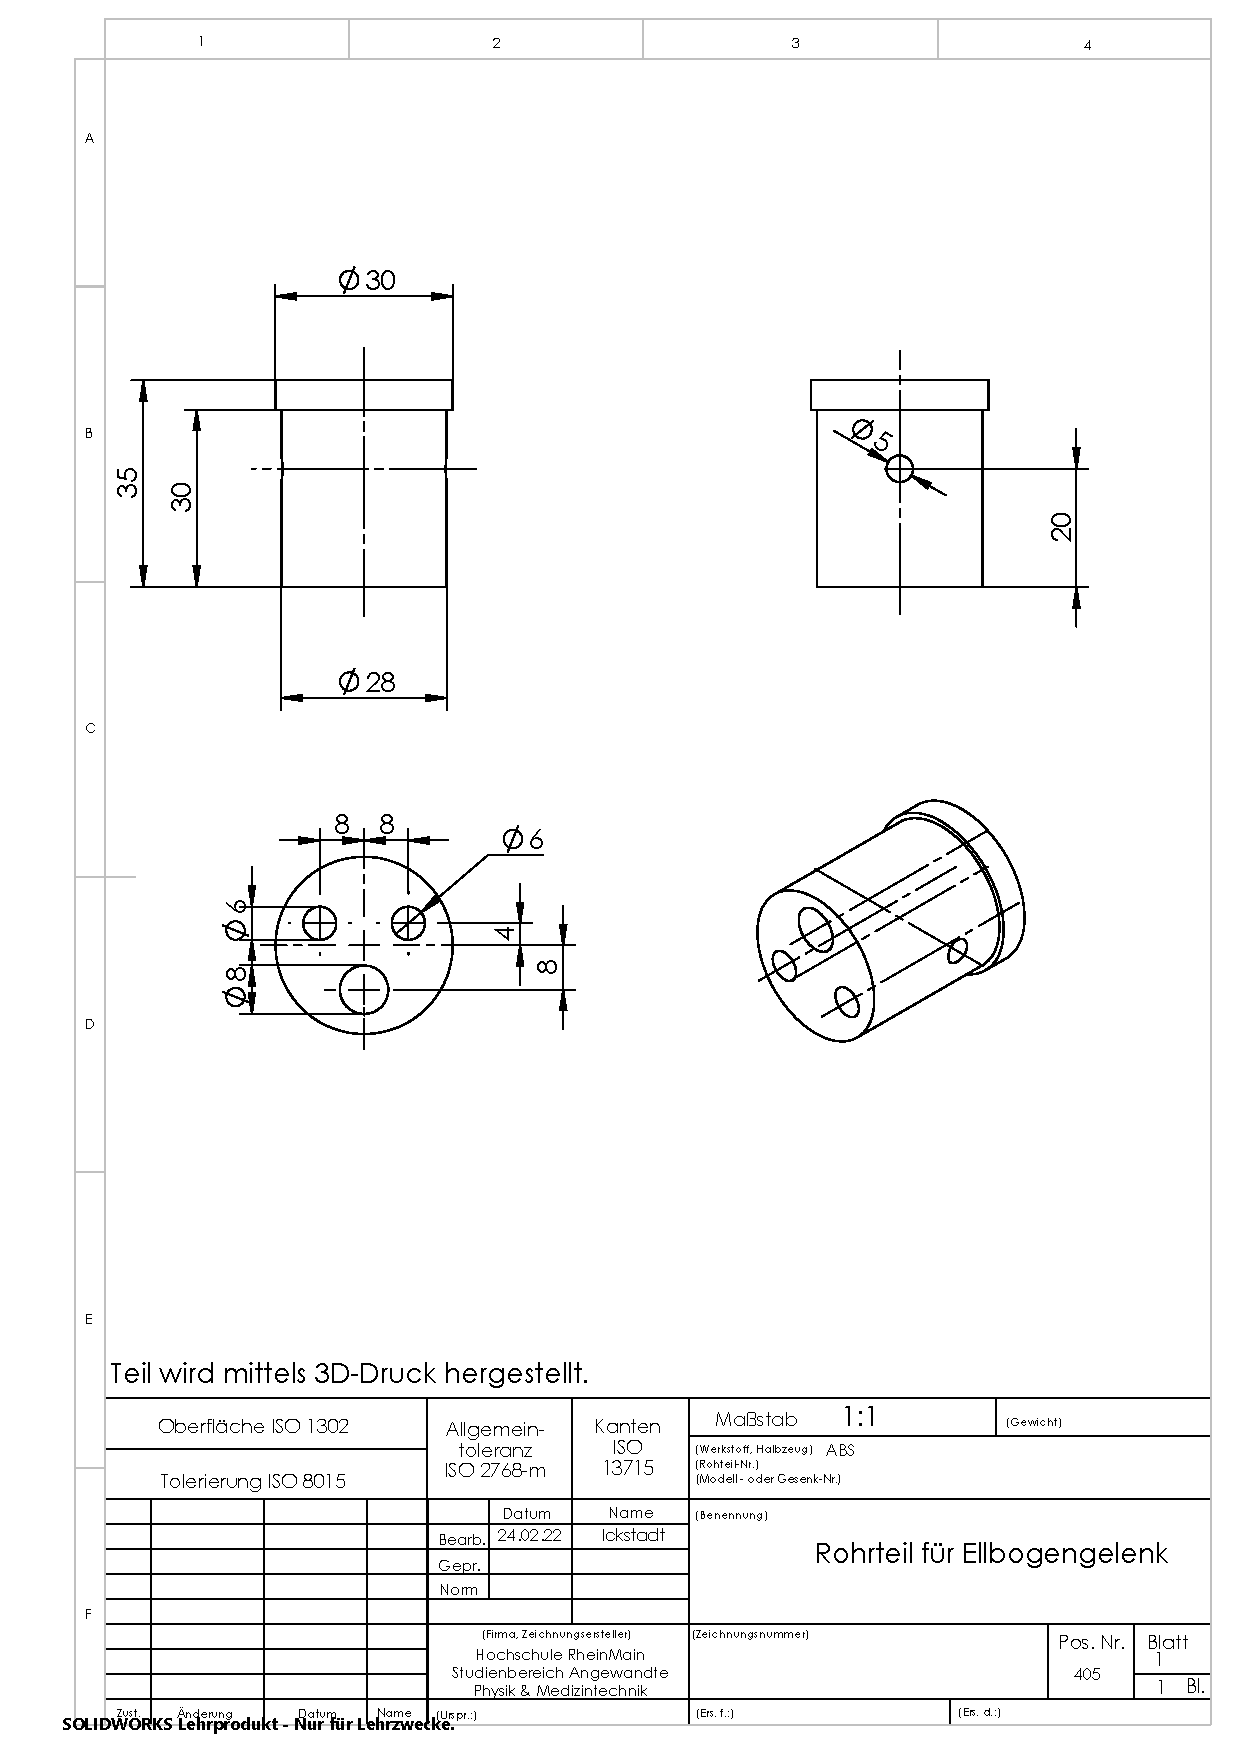
\includepdf[pages=-, angle=0, pagecommand={\thispagestyle{plain}}]{Abb/CAD/Drawings/Rohrteil-fuer-Ellbogengelenk.pdf}
% \includepdf[pages=-, angle=0, pagecommand={\thispagestyle{plain}}]{Abb/CAD/Drawings/.pdf}
\newpage
\setlength{\voffset}{-2.5 cm}
\setlength{\hoffset}{-2 cm}
\section{Generelle Stückliste und Pneumatikschaltplan}\label{sec:stueckliste und pneumatikschaltplan}
\newpage
\setlength{\voffset}{0 cm}
\setlength{\hoffset}{0 cm}
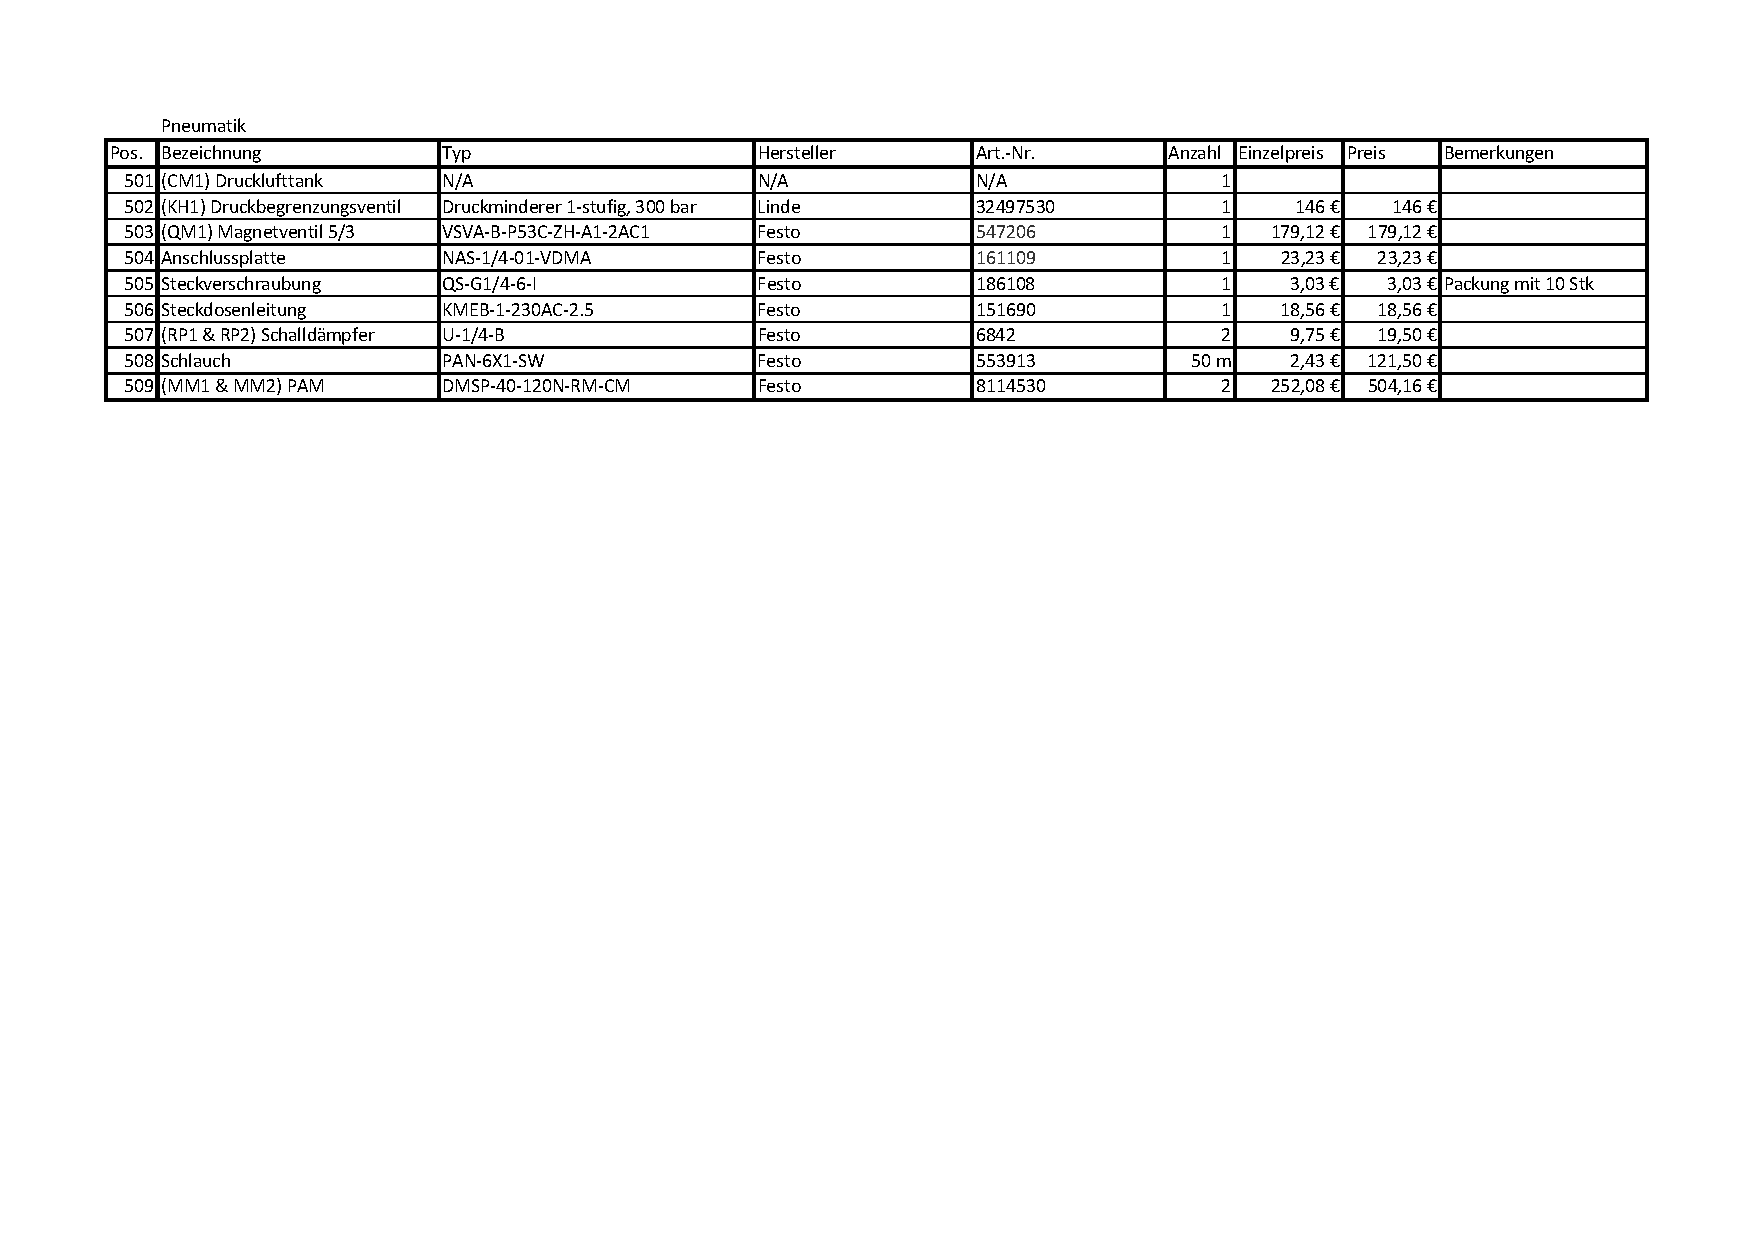
\includepdf[pages=-, angle=90, pagecommand={\thispagestyle{plain}}]{Abb/Stuecklisten/StuecklistePneumatik.pdf}
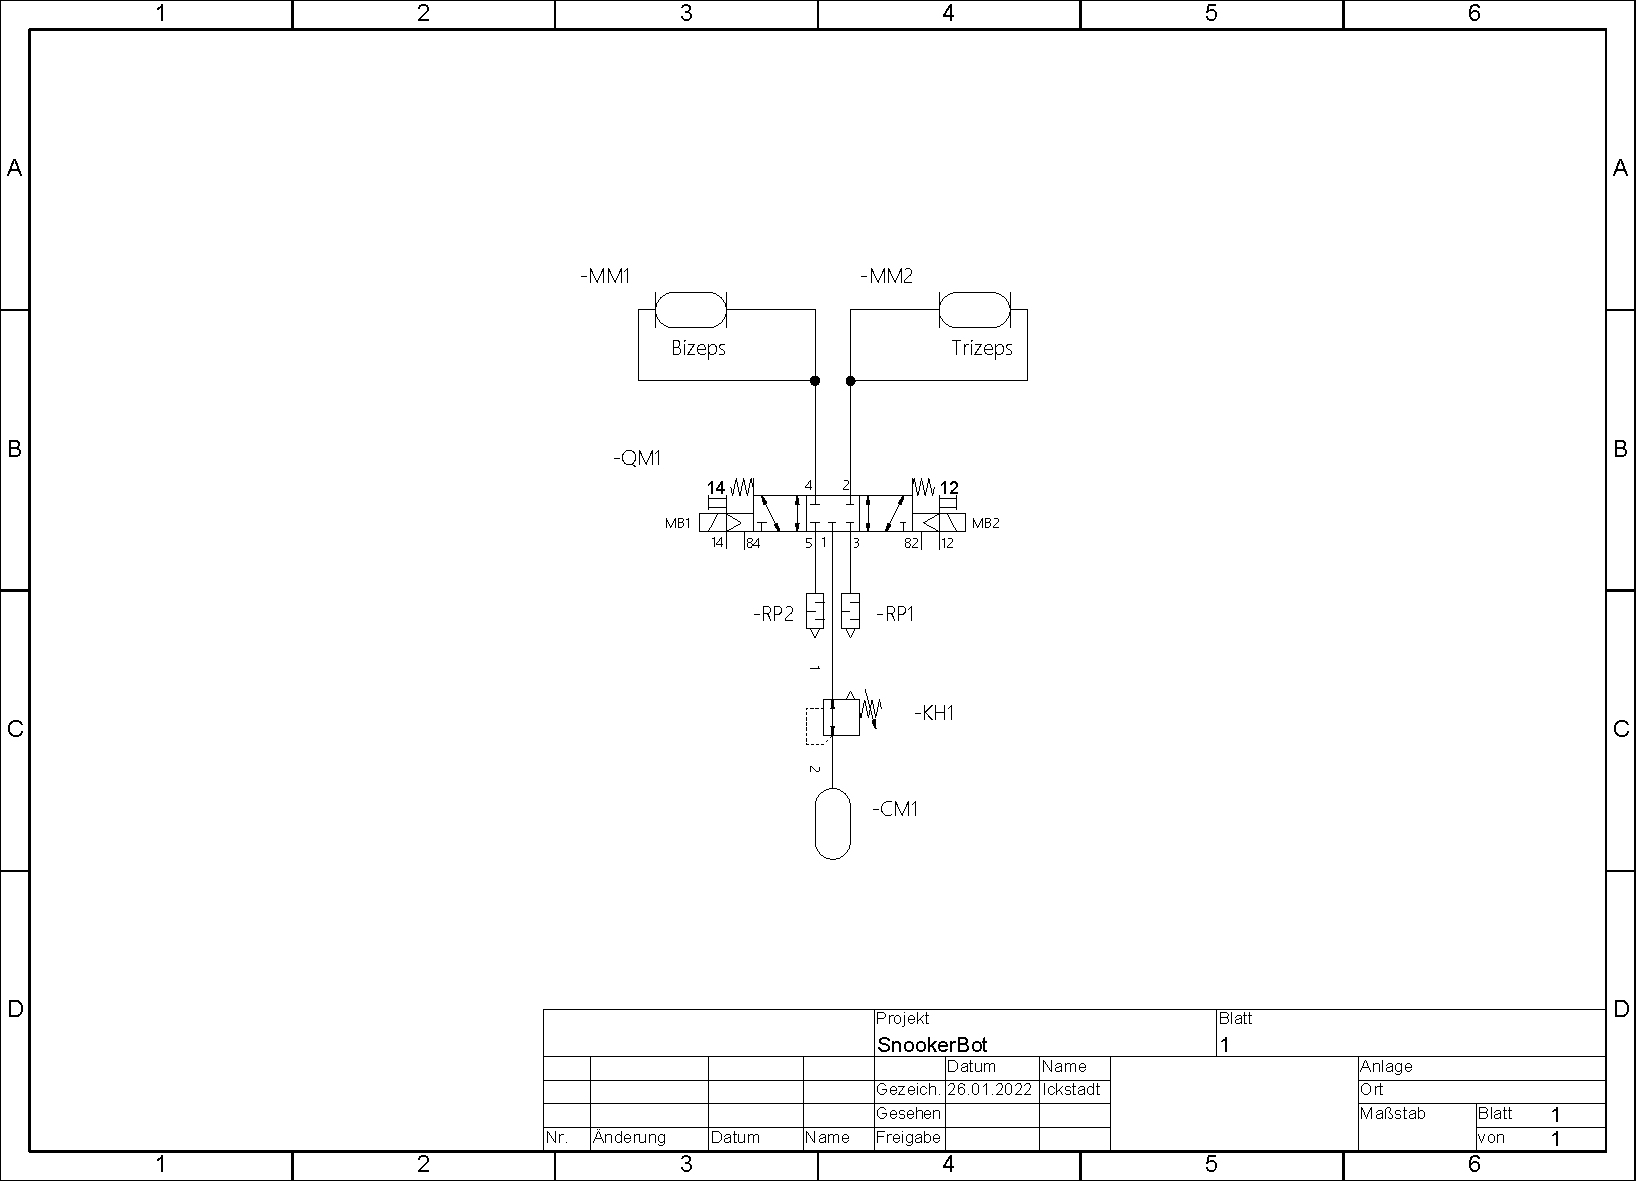
\includepdf[pages=-, angle=90, pagecommand={\thispagestyle{plain}}]{Abb/PneumatikZeichnung.pdf}
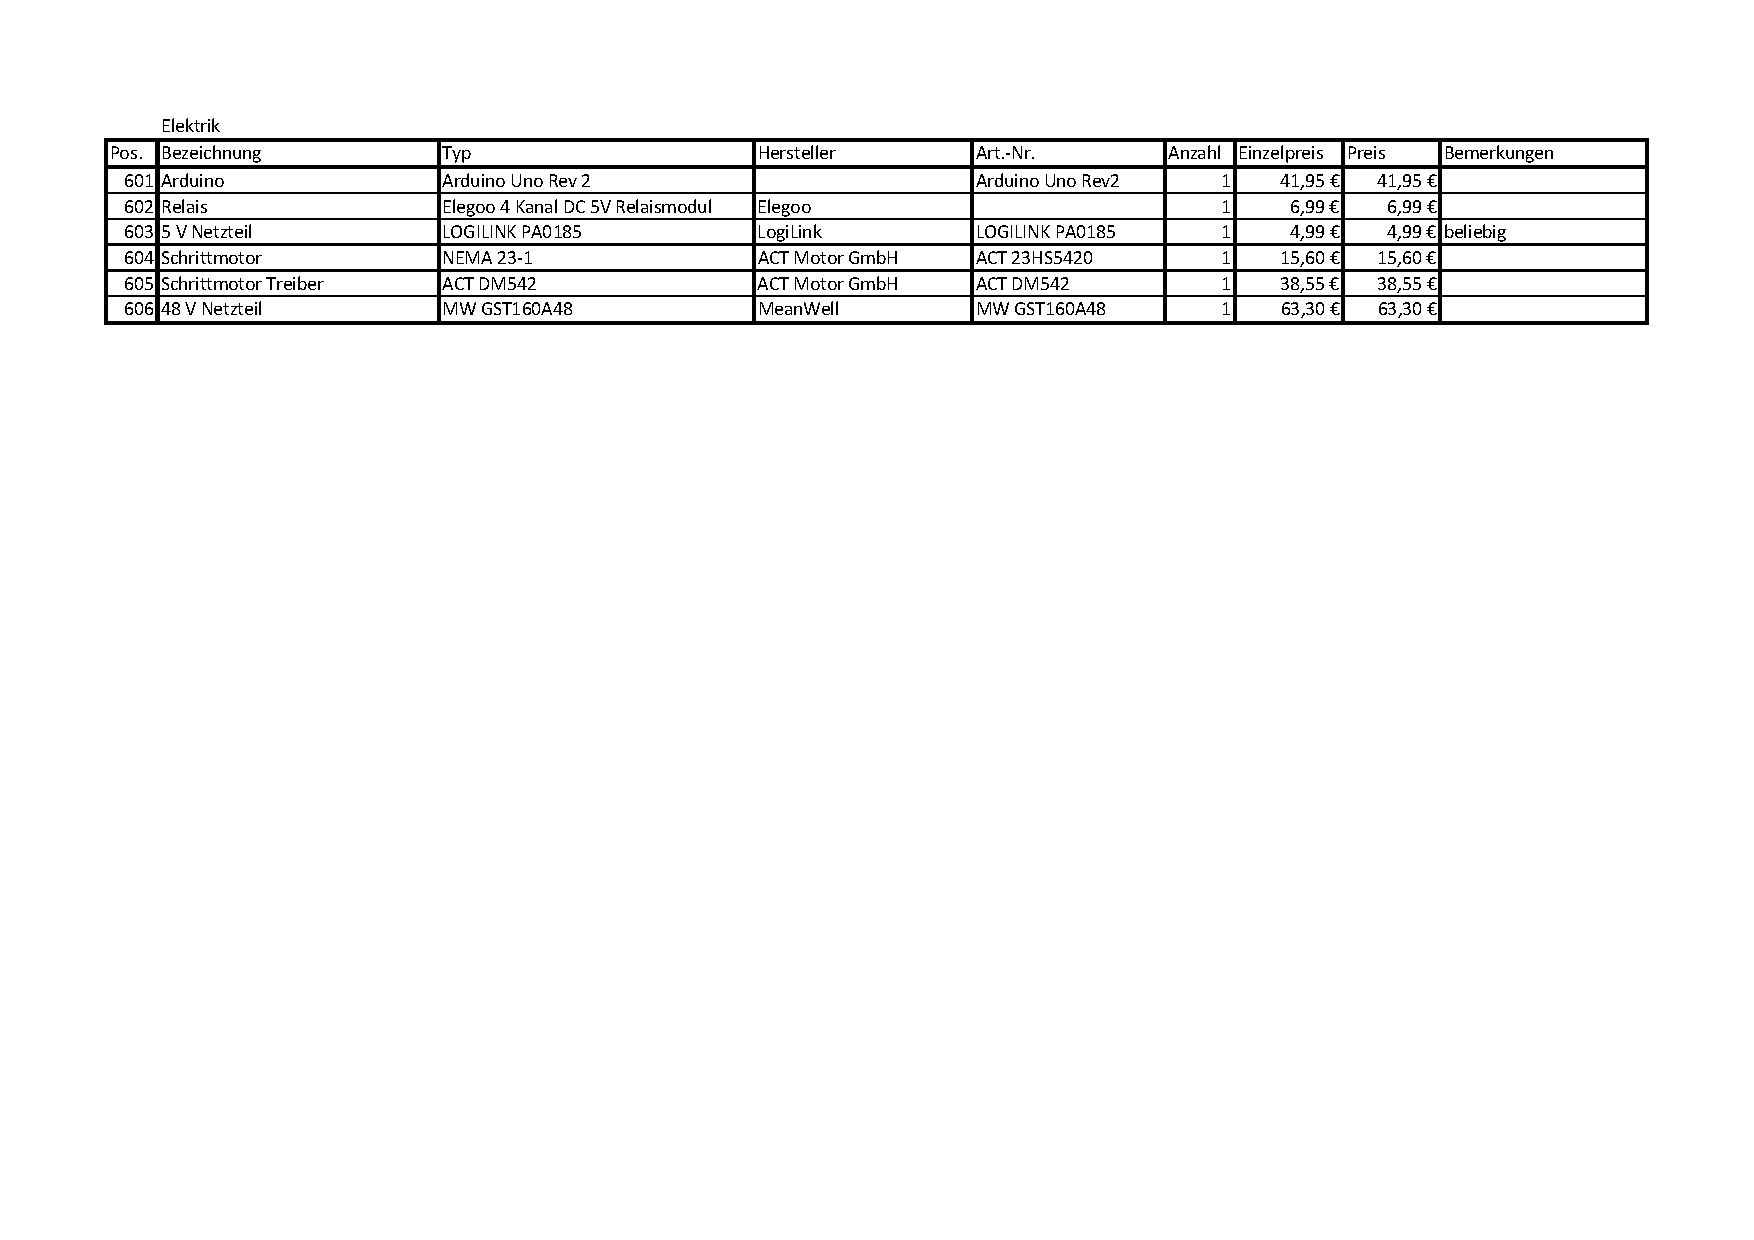
\includepdf[pages=-, angle=90, pagecommand={\thispagestyle{plain}}]{Abb/Stuecklisten/StuecklisteElektrik.pdf}
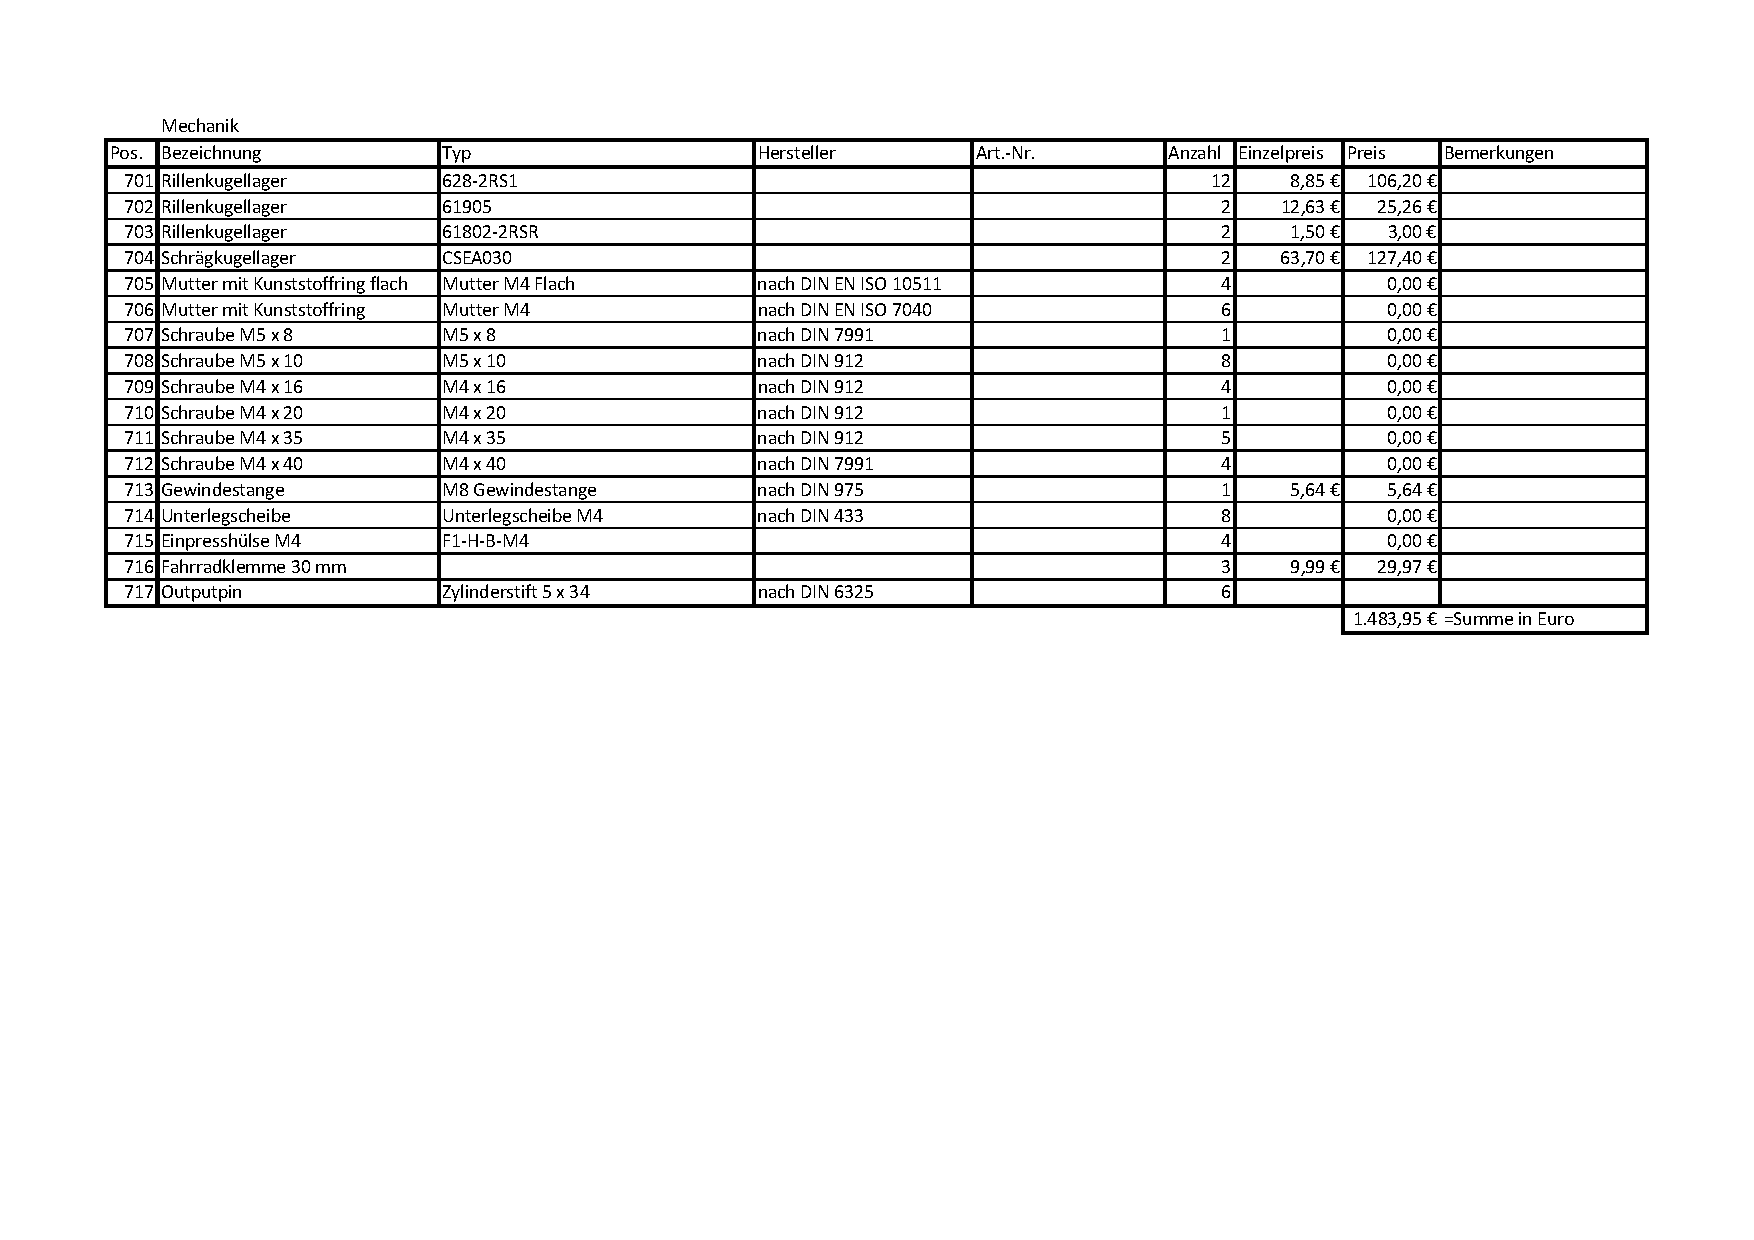
\includepdf[pages=-, angle=90, pagecommand={\thispagestyle{plain}}]{Abb/Stuecklisten/StuecklisteMech.pdf}
\newpage
\setlength{\voffset}{-2.5 cm}
\setlength{\hoffset}{-2 cm}